\documentclass{report}

%------------------------------------------------------------
% All packages are here defined
%------------------------------------------------------------
%\usepackage{mathtools}
\usepackage[table]{xcolor}
\usepackage[a4paper]{geometry}
\usepackage{vmargin}
\usepackage[english]{babel}
\usepackage[english]{varioref}
\usepackage[utf8]{inputenc}
\usepackage{graphicx}
\usepackage{array}
\usepackage{float}
\usepackage{tabularx}
\usepackage{hhline}
\usepackage{amsmath}
\usepackage{amssymb}
\usepackage{hyperref}
\usepackage{url}
\usepackage{fancyhdr}
\usepackage{setspace}
\usepackage{listings}
\usepackage{color}
\usepackage{abstract}
\usepackage{titlesec}
\usepackage{multirow}
\usepackage{datetime}
\usepackage{varwidth}
%\usepackage{svg}
\usepackage{caption}
\usepackage{epsfig}
\usepackage{blindtext}
\usepackage{xcolor}
\usepackage{enumitem}
%----------------------------------------------------
%	MARGINS
%----------------------------------------------------
\setmarginsrb  { 1.5in}  % left margin
                        { 0.6in}  % top margin
                        { 1.0in}  % right margin
                        { 0.8in}  % bottom margin
                        {  20pt}  % head height
                        {0.25in}  % head sep
                        {   9pt}  % foot height
                        { 0.3in}  % foot sep
%----------------------------------------------------------------------------------------

%-------------------------------------------------
% Colors defination
%--------------------------------------------------
\definecolor{dkgreen}{rgb}{0,0.6,0}
\definecolor{gray}{rgb}{0.5,0.5,0.5}
\definecolor{mauve}{rgb}{0.58,0,0.82}
\definecolor{navyblue}{rgb}{0.0, 0.0, 0.5}



%-------------------------------------------------
% JAVA language settings for code insertion
%---------------------------------------------------
\lstset{frame=tb,
  language=Java,
  aboveskip=3mm,
  belowskip=3mm,
  showstringspaces=false,
  columns=flexible,
  basicstyle={\small\ttfamily},
  numbers=none,
  numberstyle=\tiny\color{gray},
  keywordstyle=\color{blue},
  commentstyle=\color{dkgreen},
  stringstyle=\color{mauve},
  breaklines=true,
  breakatwhitespace=true,
  tabsize=3,
  captionpos=b
  %numbers=left,                    % where to put the line-numbers; possible values are (none, left, right)
  %numbersep=10pt
}

%----------------------------------------------------------
% Horizontal line formation
%--------------------------------------------------------
\newcommand{\Hline}{\par
  \begin{center}
   \line(1,0){400}
   \end{center}
}


%------------------------------------------------------
% heading formation for chapters and other headings
%------------------------------------------------------
\titleformat
{\chapter} % command
[display] % shape
{\bfseries\LARGE} % format
{\Huge{Chapter.\ \thechapter}} % label
{0.5ex} % sep
{
\rule{\textwidth}{1pt}%
\vspace{1ex}
\centering
} % before-code
[
\vspace{-0.5ex}%
\rule{\textwidth}{0.3pt}
] % after-code

%-------------------------------------------------------
%heading formation for Acknowledgement
%-------------------------------------------------------


%---------------------------------------------------------
% Others
%----------------------------------------------------------

\newdateformat{mydate}{\monthname[\THEMONTH] \THEYEAR}	
%\geometry{a4paper}
\renewcommand{\abstractnamefont}{\normalfont\LARGE\bfseries}


%------------------------------------------------------
% Beginning main document
%---------------------------------------------------

\begin{document}
\pagenumbering{gobble} 


%----------------------------------------------------------------------------------------
%	Title page
%----------------------------------------------------------------------------------------
\begin{titlepage}
\begin{center}


{\huge \bfseries Graph Theoretical Algorithms For }\\[0.3cm]
{\huge \bfseries Structural Comparison Of Java Source}\\[0.3cm] % Thesis title
{\huge \bfseries  And Byte Code }\\[0.3cm]
\Hline

\begin{center}
\large{Submitted By}\\[0.2cm]
\textbf{\Large{Artem Garishin}}\\[2cm]
\end{center}


\includegraphics[width=0.50\textwidth]{Figures/FH_logo}\\[0.5cm]
\textbf{\large FB2: Faculty of Computer Science and Engineering}\\[1cm]


\large \textit{This thesis presented for the degree of\\ Master of Science} \\
\textit{in the}\\[0.2cm]
\textbf{\textcolor{navyblue}{High Integrity Systems}}\\[2.5cm] % Research group name and department name

\begin{center}


\begin{varwidth}{0.8\textwidth}
\raggedright
\textbf{Research Supervisor}: {Prof. Dr. Sergej Alekseev}\\[0.2cm] % Supervisor name - remove the \href bracket to remove the link  
\textbf{Co-Supervisor}: {Prof. Dr. Matthias Wagner}\\ % Supervisor name - remove the \href bracket to remove the link  
[3cm]
\end{varwidth}\\[3cm]
\end{center}



{\large \mydate\today}\\[1cm] % Date
%\includegraphics{Logo} % University/department logo - uncomment to place it

\vfill

\end{center}

\end{titlepage}


%----------------------------------------------------------
%Declaration
%---------------------------------------------------------
%\doublespacing%
\onehalfspacing
\null\vfil
%\vskip 60\p@
\begin{center}{\huge\bf Legal Declaration\par}\end{center}
%\vskip 60\p@
\null
I declare that this thesis document is completely my own work and all used references have been clearly cited. I have not submitted this assignment in the context of an examination to any other examination board or person.\\[2.5cm]

\begin{flushleft}
Signature:\\
\rule[1em]{25em}{0.5pt} % This prints a line for the signature
 
Location, Date:\\
\rule[1em]{25em}{0.5pt} % This prints a line to write the date
\end{flushleft}


%-----------------------------------------------------------------
% Abstract 
%----------------------------------------------------------
\newpage
\pagestyle{fancy}
\fancyhead{}
\renewcommand{\headrulewidth}{0pt}
\renewcommand{\footrulewidth}{0.4pt}
\pagenumbering{Roman}
%\doublespacing
\begin{abstract}

Goal of this work is research for the optimal techniques to compare similar and at the same time different fragments of code. So far, there are two most well-known techniques of code comparison: textual-based and structural-based approaches. The textual comparison can be to some extent insufficient to analyse a difference or to find a code similarity between given pieces of code. For that reason, a structural comparison is being investigated and improved in regards with clone detection, plagiarism and code similarity.

\end{abstract}

%--------------------------------------------------------
%Acknowledgement
%-------------------------------------------------------
\newpage
%\null\vfil
%\vskip 60\p@
\begin{center}{\huge\bf Acknowledgments\par}\end{center}
%\vskip 60\p@
\null
I would like to take this time to thank Frankfurt University of Applied Sciences for all of the resources which they provided me in order to pursuing my master study in computer science and make this thesis possible.\vspace{5 mm}

\noindent I would like to express my sincere gratitude to Prof. Dr. Sergej Alekseev and Prof. Dr. Matthias Wagner for their patient guidance, encouragement and advice which they provided me throughout this thesis work.

%----------------------------------------------------------------------
% Some configurations
%-------------------------------------------------------

\newpage
\tableofcontents
\listoffigures
\listoftables

%--------------------------------------------------------
%Abbreviations
%-------------------------------------------------------
\newpage
\setstretch{1.5}
%\null\vfil
%\vskip 60\p@
\Hline
\begin{center}{\huge\bf Abbreviations\par}\end{center}
\Hline
%\vskip 60\p@
\vspace{10mm}
\null

\noindent
\textbf{AST} \hspace{24 mm}  \textbf{A}bstract \textbf{S}yntax \textbf{T}ree \\
\textbf{BCV} \hspace{24 mm}  \textbf{B}yte \textbf{C}ode \textbf{V}isualizer \\
\textbf{BFS} \hspace{25 mm}  \textbf{B}readth \textbf{F}irst \textbf{S}earch \\
\textbf{BUMC} \hspace{20 mm} \textbf{B}ottom \textbf{U}p \textbf{M}aximum \textbf{C}ommon \\
\textbf{CDS} \hspace{24 mm}  \textbf{C}ontrol \textbf{D}ependency \textbf{S}ubgraph \\
\textbf{CFGF} \hspace{22 mm} \textbf{C}ontrol \textbf{F}low \textbf{G}raph  \textbf{F}actory \\
\textbf{DDS} \hspace{24 mm}  \textbf{D}ata \textbf{D}ependency \textbf{S}ubgraph \\
\textbf{MBWM} \hspace{18 mm} \textbf{M}aximum \textbf{B}ipartite \textbf{W}eighted \textbf{M}atching \\
\textbf{PDG} \hspace{24 mm}  \textbf{P}rogram \textbf{D}ependecny \textbf{G}raph \\
\textbf{SCV} \hspace{24 mm}  \textbf{S}ource \textbf{C}ode \textbf{V}isualizer \\
\textbf{TDMC} \hspace{20 mm} \textbf{T}op \textbf{D}own \textbf{M}aximum \textbf{C}ommon \\
\textbf{TC} \hspace{27 mm}   \textbf{T}ext \textbf{C}ompare \\




%------------------------------------------------------
% Example chapter
%------------------------------------------------------

%\chapter{Example}
%\section{Section}
%This is section heading
%\subsection{Sub Section}
%This is sub section

%------------------------------------------------------
% 1st Chapter Introduction
%------------------------------------------------------

\newpage
\pagenumbering{arabic}
\onehalfspacing
\large

\chapter{Introduction}
The code maintenance is one of the most important component in software project development. It is obvious, that the whole development process is based on re-usage and adjusting of existing code fragments. But practically, it is observed, that mostly the code duplication and further appliance are not proper used. Large software projects are developed by many people for years and at some point there are problems in applications since the code was not proper supported. These issues, like the code duplication and then following re-usage by copy-pasting with or without any modifications are a well known problems in computer software maintenance.
\\
These problems of disordered code usage originally come from tendency of directly copy fragments of code that implement something similar for the personal needs and by performing small correction. The code is adapted to the new applications and consequently the code is already reused. To copy a code fragment (which may be already tested for functional purposes) is easier and faster than to implement the code from scratch.
\\
Many studies say that about 5 to 20 percent of a computer software systems can contain a duplicated code fragments. One of the major disadvantages of such duplicated code fragments is that in case of bug detection in a code fragment itself, all the other fragments similar to it should be investigated to check the possible existence of the same bug in the similar fragments. Another problem is the code redundancy, particularly unknown pieces of reusable code are located in different places that makes code uncomprehending for further development. 
\\
In addition, another no less important problem nowadays is plagiarism detection. Most occasions of plagiarism are found in documents are typically articles, reports or essays. Nonetheless, plagiarism can be found in any field, including scientific papers, art designs and source code. In this work, objectively is a question about source code duplication and their methods to find out similar or same fragments of source code. Java is one of the most well-known of programming languages that used in many open-source projects available in world open network. Indeed, the majority of them are not developed from scratch and there are many methods and functions that have been created by copy-pasting and consequent code adjustment.
\\
The clone detection and following re-factoring of the duplicated code is theme for discussion in software maintenance. Although, practically restructuring code without changing its external behaviour of certain clones are not desirable and there are a risks when these duplication have been removed. However, it is widely agreed, that clones should at least be detected and somehow taken into consideration.
\\
Modern methods to compare of code fragments are used to analyse codes changing, to explore the development process and to optimize the code implementation. Basically, in actual tools or plug-ins only text compare methods are used, for example embedded text-to-text compare feature in Eclipse IDE. In several cases this is not full sufficient to define clones or moreover to comprehend where these code clones located. Sometimes, another techniques can be very helpful for such purposes like structural code comparison.
\\ 
Portions of the source code for some proprietary software are leaked to the Internet. This could be an evidence of the frequently made assertion by proponents of open source that it is difficult to keep source code in secret. The most remarkable examples of code clones have open source projects as MySQL and PostgreSQL database management systems. The same way open-source operation systems Linux and FreeBSD have been implemented. The table \ref{table:products-compare} presented from the research of clone detection tool in \cite{CP-Miner} shows the figures of code clones these projects.

\begin{table}[h]
\centering
\begin{tabular}{|c|c|c|}
\hline
\rowcolor[HTML]{C0C0C0} 
\multicolumn{1}{|l|}{\cellcolor[HTML]{C0C0C0}\textbf{Project}} & \multicolumn{1}{l|}{\cellcolor[HTML]{C0C0C0}\textbf{Number of segments}} & \multicolumn{1}{l|}{\cellcolor[HTML]{C0C0C0}\textbf{Copy-pasted \%}} \\ \hline
Linux                                                          & 198,605                                                                   & 23.0\%                                                               \\ \hline
FreeBSD                                                        & 153,230                                                                   & 20.4\%                                                               \\ \hline
Apache                                                         & 6,196                                                                     & 17.7\%                                                               \\ \hline
PostgreSQL                                                     & 16,662                                                                     & 22.2\%                                                               \\ \hline
\end{tabular}
\caption[Statistical data of clones detected in open-source products]{The table shows statistical data: number of overall code segments in open-source software products and their percentage of copy-pasted segments}
\label{table:products-compare}
\end{table}
As presented in the table \ref{table:products-compare}, in Linux and FreeBSD, there are around 200,000 and 150,000 copy-pasted segments without any modifications. This percentage composes circa 20\% of the whole written copy-pasted code scattered in the project. In other words, the code quarter of these four software products is practically identical and has same application logic.

%-----------------------------------------------------
% 2nd Chapter: Description of problem
%-----------------------------------------------------
\newpage	
\chapter{Description of problem}
\label{cha:Description}
In this chapter an issue of actual topic in the master work is being explained. As usual, a comparison of two code fragments considers a selection of classes, functions or loops to be in between compared. Thereby, a compare can be counted as examinations of two pieces of code, in the most convenient way - methods or functions. They can have a similar implementation or alike syntax at first sight, however these two pieces of code are different. As well, the pieces of code can be completely varied and therefore this variety needs to be investigated. 
\\
There are many purposes to compare a code, to find out a similarity or to determine a difference between them. One of the option is search for plagiarism in case code can be taken from external source and a names variables, classes and functions have been changed. This case called code clone, by reason that has identical implementation, i.e the same logic. In addition to the general plagiarism detection it can be improved to look out for similar code in large projects. This is needed to search out for an equal code chunks and by that reduce the code superfluity.

\section{Insufficiency of textual comparison approach}
Possible result of this thesis is research of concept and idea to find out code difference using graph theory and potential suggestions to upgrade existing practises of code comparison. To get started, the introduction why the textual comparison is not sufficient, a small example demonstrates, what kind of result delivers normal text compare. The listing below provides an example of two code clones.

 \newpage
\begin{lstlisting}
		public void method1(){
		if(i > 1) i++;
	}
	
	public void method2(){
		if(i > 1) 
		i++;
	}

\end{lstlisting}
	
In this example there are two pieces of code presented methods \texttt{method1} and \texttt{method2} in Eclipse compare editor. One enter symbol after line \texttt{if(i > 1)} takes place in \texttt{method2}. Therefore, the result of the codes in textual image looks different, there is a highlight of string mismatch. Even a calculation of statistic how much code is different, the a preliminary answer two rows is wrong and is not fully precise.
Using trivial text-based approach of compare, only these gap will be found, however, this difference does not play any role regards to application logic. The suspicious piece, for example \texttt{method2} of code can be written in one string and textual compare editor is not able to deliver proper results.

\begin{figure}[h]
  \centering
  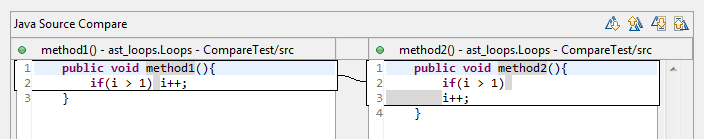
\includegraphics[scale=0.6]{Figures/introduction/intro-code-example}\\[0.1cm]
  \caption[Simple textual comparison example in Eclipse compare editor]{The simplest example of text-to-text comparison indicating that text compare sometimes is not enough to investigate code difference, however there are no changes regards the application logic.}
  \label{fig:intro-code-example}
\end{figure}

\section{Structural graph comparison is NP-complete problem}

Since the code is a clear text from abstract point of view, the code difference can be introduced as a composition of two compared objects and highlighted and imposed snippets on both texts. This trend of comparison called textual compare when strings of code are collated to each other and mismatches between them are revealed. Such way to discover a difference has some drawbacks. The chapter Existing Methods of Code Comparison, section Text-based techniques \ref{sec: text_tech} discloses their shortages. Another more optimized way is approach using graph theory, or by another words the structural comparison.
\\
The structural comparison stands for comparing data graphs structures. There are some techniques of graph creation from java source code. Generally, the data structure extracted from source code are graphs, an examples are flowcharts or dependency graphs. In order to find some structural similarities, this two created graphs must be somehow compared for isomorphism, so-called graph similarity. For this purpose there is an amount of existing algorithms to figure out graph isomorphism. But unfortunately, their execution time is exponential complex and in some bound not a proper solution. Nevertheless, tree data structures can be compared in polynomial time, that is not reachable for graphs. The graphs can contain loop inside, i.e. edges from parent follow via other nodes to its parent node, or back edges, that are an edges that connects a vertex to itself. Basically, these types of graphs as program flowchart or program dependency graphs are circular graphs. 
\\
If two graphs are compared with each other to figure out graph isomorphism then it is NP-problem. Graph isomorphism between two graphs $G_{1}$ and $G_{2}$ is a bijection between the vertex sets $f: V(G_{1}) \rightarrow V(G_{2}) $ such that \\ $ \forall v, w \in V(G_{1})$:  $ \{v,w\} \in E_{1} \iff \{ f(v), f(w)\} \in E_{2}$. 
\\
In the complex theory the worst case running time of all known algorithms is of exponential order, and just for certain special types of graphs, polynomial-time algorithms have been devised \cite{graph_isomorphism_is}. Maximum common sub-graph isomorphism is an optimization problem that is known to be NP-hard. The formal description of the problem is as follows:
there are two input graphs, respectively the maximum common sub-graph isomorphism MCSGI($ G_{1}, G_{2}$):

\begin{itemize}
	\item     Input: Two graphs $ G_{1}$ and $G_{2}$.
	\item     Question: What is the largest sub-graph of  $ G_{1}$ isomorphic to a sub-graph of  $ G_{2}$ can be found?
\end{itemize}

The associated decision problem, i.e., given $ G_{1}$ and $ G_{2}$ and an integer $k$, deciding whether $ G_{1}$ contains a sub-graph of at least $k$ edges isomorphic to a sub-graph of $ G_{2}$ is NP-complete \cite{graph_isomorphism_is}.This type of graph comparison is very expensive from a computational point of view and thus an action must be taken into account to reduce the domain of comparison before performing the actual comparison. To avoid this problem, luckily, a tree comparison is able to be executed in polynomial time. Moreover, there are some existing algorithms to investigate trees for isomorphism that presented in this paper.\\
Thus, there are no deterministic algorithms to compare graphs because of loops inside. In this case, the input code can be transformed into flowchart graph firstly, after the graph creation, it must be converted into tree, using non-trivial pre-process actions, for example, removing back edges. The back edges in the input graph are edges, which point from a node to one of its ancestors. Another approach is usage of AST trees obtained from source code. In fact, none of extra operations like, removing of back edges required that can beneficial to use AST trees.
\newpage
Under these circumstances the following techniques are researched and presented in the paper.
After the prerequisites the following questions can be inquired:
\begin{enumerate}
 \item How to optimize the search of code for similarity?  
  \item How to compare these trees to get reasonable results?
  \item How to reference code pieces and nodes, respectively how to put the code difference by the most elegant way?
\end{enumerate}

Regards to the first question, the concept of idea is described in chapter \textbf{Techniques to normalize AST trees} \ref{cha:ast_normal}. The second question comprehends existing algorithm and their combination and improvements in chapter \textbf{Maximum common subtree isomorphism algorithms} \ref{cha:algorithms-to-compare}. The last issue concerns about process to lead back the result using logic of code and is stated in chapter \textbf{Text comparison improvements} \ref{cha:text-improvement}.

%-----------------------------------------------------
% 6th Chapter: Graph transformation algorithms
%-----------------------------------------------------
\chapter{Existing comparison methods for plagiarism detection}
\label{cha:methods}
\section{Plagiarism detection methods}
\label{sec: plagiarism_methods}

Task of plagiarism detection is an identification of text's similarity. Thus, a research of existing methods is useful for this work regards code's comparison.
The citation from \cite{software_clone_detection}:
\begin{quote} Detection of plagiarism can be either manual or software-assisted. Manual detection requires substantial effort and excellent memory, and is impractical in cases where too many documents must be compared, or original documents are not available for comparison. Software-assisted detection allows vast collections of documents to be compared to each other, making successful detection much more likely.\end{quote}

\noindent
Mostly the task of plagiarism detection is considered for many fields, like text documents, software and source code. In this chapter source code plagiarism is being reviewed.
According to the article of Chanchal Kumar Roy and James R. Cordy \cite{software_clone_detection}, source-code similarity detection algorithms can be classified as following:
\begin{itemize}
	\item Text-based Techniques
	\item Token-based Techniques
	\item Tree-based Techniques
	\item PDG-based Techniques
	\item Metrics-based Techniques
\end{itemize}
According to this research the mostly useful and leading methods are described in this chapter. The following conclusions take place after every method to overview pros and cons of them and to gain a profit to reform the existing algorithms. 

\section{Text-based Techniques}
\label{sec: text_tech}
Text based techniques are widely used to compared pieces of text. For this purpose they can be valuable to compare java source code, but sometimes insufficient. This section shortly explains how it functions and derived advantages and disadvantages from chapter experiments \ref{cha:experimental} are characterized. Used technique in text-to-text comparison applies so-called tree suffix algorithm, designed to compare strings. General idea of this suffix tree comparison algorithm: the code is split into strings, afterwards from these strings a suffix tree is being built, then using sub-suffix algorithm performs a search for substring from one code fragment to another. Building such kind of tree allows to find a sub-string in given string within $O(m)$ complexity, where $m$ is the length of the sub-string (but with initial $O(n)$ time required to build the suffix tree for the string, where $n$ is input string). Thus the algorithm is being applied for normalized text after steps above. 
\vspace{5mm}
\begin{figure}[h]
  \centering
  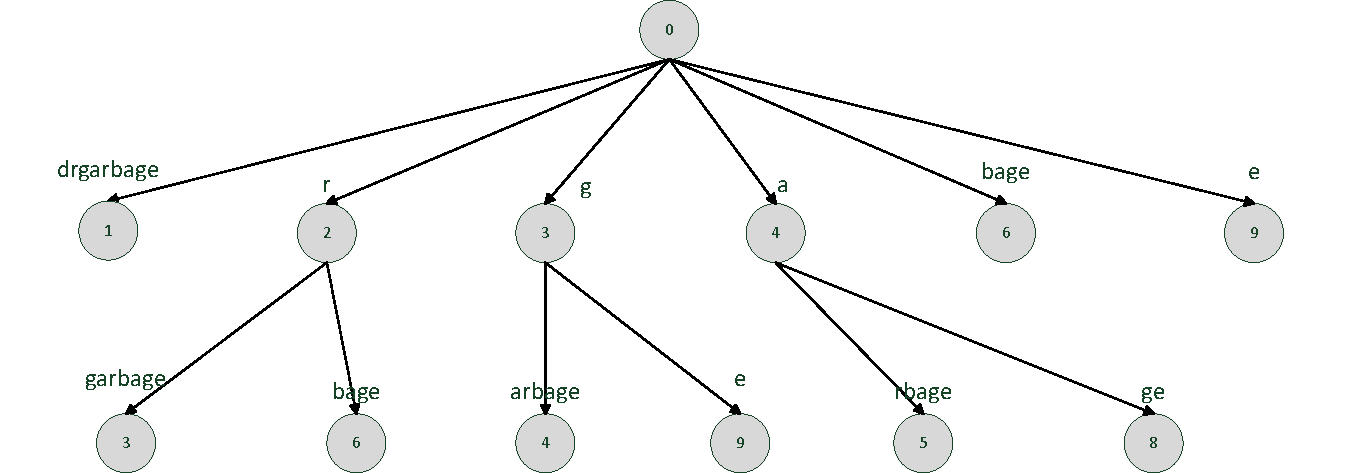
\includegraphics[scale=0.65]{Figures/exist-alg/suffix-tree.pdf}\\[0.1cm]
  \caption[Example of suffix-tree data structure decomposed on word ]{Example of suffix-tree data structure decomposed on word \textbf{drgarbage}. The number inside of each node indicates index of the first letter. The text under each node means a sub-string depending on parent node.}
  \label{fig:suffixtreeexample}
\end{figure}

The figure \ref{fig:suffixtreeexample} shows the built suffix-tree based on word \textbf{drgarbage}. The tree has been created by so proficient way, that sub-string search is minimized. Without such tree structure the worst case of search considers to iterate all possible combinations, that is $O(n^2)$. For example, to find a whether the word $garbage$ enters in the $drgarbage$, the algorithm looks first for the first letter of search string - $g$, it was found, then there only 2 possible combinations to consider for exact match, since node $g$ has two child-nodes. The rest of search words is sliced till $arbage$. If there is a leaf-node with such content then the word is found. For instance, $garbaga$ cannot be found since there are no leaf node with exact the matched content.
\\
The text comparison splits each $i$ line of code and compare the string with $i$ line of code of other fragment. From the first string the suffix tree is built. The second line of code as a search-string is interpreted. The suffix tree is traversed looking for search string occurrence. From performed chapter of experiments \ref{cha:experimental} the next feedback of this approach can be derived. \\
Advantages of text-to-text comparison using tool Eclipse compare editor:
\begin{itemize}
	\item The difference direct in text represented.
	\item Every small mismatch is noticed and highlighted.
	\item High performance due to optimal formed suffix tree, that the match of search string is for $O(m)$ complexity executed, where $m$ is length of searched sub-string.
\end{itemize}
Disadvantages of text-to-text comparison using tool Eclipse compare editor:
\begin{itemize}
	\item If lines of the same command are different, comparison declare it as a mismatch.
	\item Changing the order of command or variable's names bring almost full mismatch.
	\item Supposing that the sequence of commands and names of variables have been changed or modified then output text-highlight result is too jumbled.
\end{itemize}

In order to avoid line's mess, the graph theory can be very helpful to make an application logic more independent from text, therefore to improve quality of text difference representation. The paragraph \ref{cha:text-improvement} interprets an idea how AST trees assist to specify precisely match/mismatch of command statements. This kind of algorithm is a beneficial to compare clear texts, that do not have logic while the java code does.

\section{Token-based Techniques}
\label{sec: tocken_tech}

Using this technique the input code is firstly prepared with lexical analyzer. The entire code is lexed, parsed and transformed into sequence of tokens. This principle is advanced text-to-text comparison concept with steps before text comparison starts the preparation of code includes following steps:
\begin{enumerate}
  \item Comments Removal: Ignores all kinds of comments in the source code depending on the language of interest.
  \item Whitespace Removal: Removes tabs, and new line(s) and other blanks spaces.
  \item Normalization: Some basic normalization might be applied on the source code.
\end{enumerate}

One of the leading token-based techniques is CCFinder from Kamiya\cite{tocken_kamiya} research. Firstly, each line of source files is divided into tokens by a lexer and the tokens of all source files are then concatenated into a single token sequence. The token sequence is then transformed, tokens are added, removed or changed based on the transformation rules of the language of interest aiming at regularization of identifiers and identification of structures. 
After that, each identifier related to types, variables, and constants is replaced with a special token\cite{tocken_kamiya}. This identifier replacement makes code fragments with different variable names clone pairs \cite{tocken_kamiya}. A suffix-tree based sub-string matching algorithm is then used 
to the similar sub-sequences on the transformed token sequence where the similar sub-sequence pairs are returned as clone pairs/clone classes\cite{tocken_kamiya}. When the clone pair class is obtained according to the token-sequence, the original code must be mapped regards to clone pair/clone class information. Data pre-processing and algorithms steps:
\begin{enumerate}
  \item \textbf{Lexical analysis} - each line of code is divided into tokens depending on programming language. The tokens are parsed via lexical analyzer which performs formatting of tokens, the rules described above are reconstructing the source code.
\item \textbf{Transformation}  - the process includes two sub-processes. During the sub-processes the meta-information regards mapping to original source code is kept. Thus the original code is restructured without loss of link-identifiers.
  \begin{enumerate}[label*=\arabic*.]
    \item \textbf{Transformation according to determined rules} - the token sequence is reorganized pursuant to some rules. One of them is conversion of compound block. For example the code: \texttt{if(i == 1) i = i + 1;} is being transformed into: \texttt{\textbf{if(i == 1) \{i = i + 1;\}}} covered within brackets. All other rules can be programming language dependent.
    \item \textbf{Parameter replacement} - each identifier related to types, variables and constant is replaced with special token\cite{tocken_kamiya}.
  \end{enumerate} 
  \item\textbf{Match detection} - the token sequences are searched for equivalent pairs and marked as clones with suffix-tree algorithm [\ref{sec: text_tech}]. Each clone is divided by indices in four parts: LeftBegin, LeftEnd, RightBegin, RightEnd. These metrics are indices of leading clone for mapping for according positions in the following clone.
  \item\textbf{Formatting} - the clones in original code are highlighted according results from previous step.
\end{enumerate}
These results followed by \cite{tocken_kamiya} provide confirmatory evidence that native text comparison [\ref{sec: text_tech}] can be significantly improved. After the data pre-processing contributions this is more suitable for compare code chunks, but not clear text. Simple based normalization of code structure, namely transformation in tokens and code editing in order not to compare useless fragments brings better results as compare to native text comparison [\ref{sec: text_tech}]. 


\section{Tree-based Techniques}
\label{sec: tree_tech}
The research from Chanchal Roy \cite{software_clone_detection} offers an alternative to figure out differences using trees derived from logic of code itself. The complex trees are formed from source code and parsed to find mismatched nodes. The most remarkable distinction between text-to-text compare and trees is logic of tree building. In other words, the text compare assumes also a suffix-tree creation, however this technique is based on input strings, i.e the structure of the tree depends on letters and sub-string \ref{sec: text_tech} not taking into consideration the code logic. The alternative tree approach is tree creation directly from source code, based on programming language. It encompasses building a branch of trees not by one string line, but by a combination of programming command structures. Such logic of tree creation called Abstract Syntax Tree (in short, AST). The abstract syntax tree analysis is more accurate than a line by line analysis or programming language token based approach \ref{sec: tocken_tech} due to the fact that it builds the abstract syntax tree.\\
The proposed clone detection solution from \cite{flavius} can be organized into few steps:
\begin{enumerate}
	\item Parsing via source code and create non-optimized standard AST tree.
	\item Each sub-tree of AST tree is hashed and grouped by in different buckets based on their hash value. 
	\item Apply the clone detection algorithm that three sub-algorithms:
		\begin{enumerate}[label*=\arabic*.]
		\item Basic Algorithm finds sub-tree clones compares every sub-tree with another sub-tree for equality. The algorithm uses parsing both AST trees finding out clones with exact equality and excludes the possibility to find near-miss clones. The complexity of algorithm offered from Baxter \cite{baxter} is 
$ O(N^3)$. This can be reduced using hash-value in node parents of sub-tree. Thus each parent node keeps a hashed value about sub-tree itself. For example, a parent node contains following tree structure: \texttt{for(int i = 1; i <= 10; i++ )\{ b = b + 1; \}} that represents a complex sub-tree. The hash-value of structure is \texttt{f4caf1dd3e33c53d971f0e18f72249e0}. During tree traverse the hash values of corresponding nodes are compared. If these hash values are same there is no need to check the whole sub-tree. Otherwise sub search is being further proceed. This technique is used to optimize search of equal sub-structures between AST trees. In most cases it contributes up to $30\%$ performance, since searched projects keep clones.
		\item Sequence Detection - is a part of clone detection the algorithm that handles the detection of code clones within sequences of statements or declarations \cite{flavius}. When parsing a source code fragment, all sequences are stored in a sequence list for future usage. The first step named subsequence algorithm, takes care of detecting code clones inside each sequence, and verifies if two sub-sequences of the same sequence are clones.	
		\item Generalization algorithm - the algorithm takes care about detection near-miss clones. It verifies whether the parent nodes of detected clones belong to near-miss clones.
		 \end{enumerate} 
\end{enumerate}

\begin{figure}[h]
  \centering
  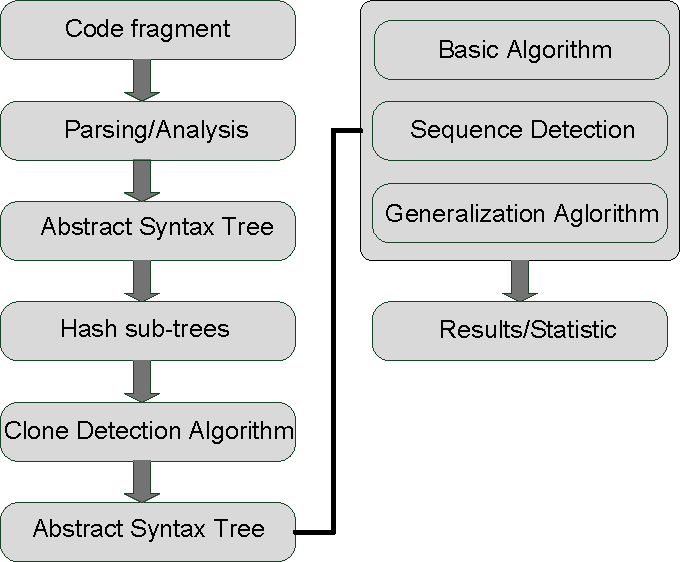
\includegraphics[scale=0.75]{Figures/exist-alg/ast-scheme2.pdf}\\[0.1cm]
  \caption[General steps of algorithm to compare code with AST tree]{The flowchart demonstrates general steps of code comparison with AST trees. Once the Abstract Syntax Tree has been created, a sequence of algorithms is applied.}
\end{figure}

In summary, tree-based approach is the most flexible tool to compare source code because only this fragment of code has a syntax and structure. Consequently, a flexible tree can be built based on syntax itself. \\
Advantages of Abstract syntax tree comparison:
\begin{itemize}
	\item Possibility to investigate for clones in sub-expressions on high abstract level
	\item Semantic analysis during tree assembling 
	\item Independence form comments, spacing, or other non-semantic changes
\end{itemize}
Disadvantages of Abstract syntax tree comparison:
\begin{itemize}
	\item Execution time, comparing sequences of trees the computational process is $O(N^4)$. But due to hashing of buckets it can be significantly reduced.
	\item Complexity of algorithms to parse trees and figure out clones.
	\item So far this algorithm have been used only to identify clones and add/remove sequences of clone to optimize projects. For small examples of code there are yet an algorithm to represent clones textually. This concept is described in section \textbf{Text comparison improvement with AST trees} \ref{cha:text-improvement}.
	\item The level of abstraction is not so high to handle application process of variables. For example, swapping of command changes the final result, however AST does not care about variable data flow.
\end{itemize}
To conclude this way of compare, as described above, it allows to differ even small clones between two pieces of code. This technique is not suitable for pure text since text has no logic and structure. AST tree based technique is not fit with java byte-code since the byte-code has not so much complex structure to form an AST tree. The shortage of such approach may be that it does not consider data flow process. Perhaps, that same clone is located under another statement therefore it makes the algorithm not able to same branch of clone.


\section{PDG-based Techniques}
\label{sec: pdg_tech}
PDG based techniques for clone detection is most suitable to detect for non-contiguous code clones while other clone detection technique as AST in section \ref{sec: tree_tech}, text and token methods are not. The most remarkable difference of this approaches is logical content of graph, therefore the dependencies among variables and methods. This method sets an effective testing to discover and locate the redundant functional modules and the unreachable paths based on dependency relationship.
\\
A program dependency graph (in short, PDG) is a directed graph $ G = (V, E)$ contains the control flow and data flow and represents the dependencies between program elements (statements). Respectively a PDG nodes $V_{i}$ is a program element and a PDG edge $E_{i}$ indicates a dependency between two nodes. PDG is considered as a combination of two different layer sub-graphs: a data dependence sub-graph (in short, DDS) and a control dependence sub-graph (in short, CDS).
After PDG graph creation, a matching algorithm is applied to find a similar sub-graphs which are returned as clones. \newpage

\begin{lstlisting}[numbers=left, numbersep=-5pt, caption=Sample of java method to be extracted into PGD graph.]
    private static String sample(){
 		   String text = null;	
		   int i = 0;
		   while(i < 10){
				i++;
				text.compareTo("my text");
				text.trim();
		}
		return  text;
	} 
\end{lstlisting}

\begin{figure}[h]
  \centering
  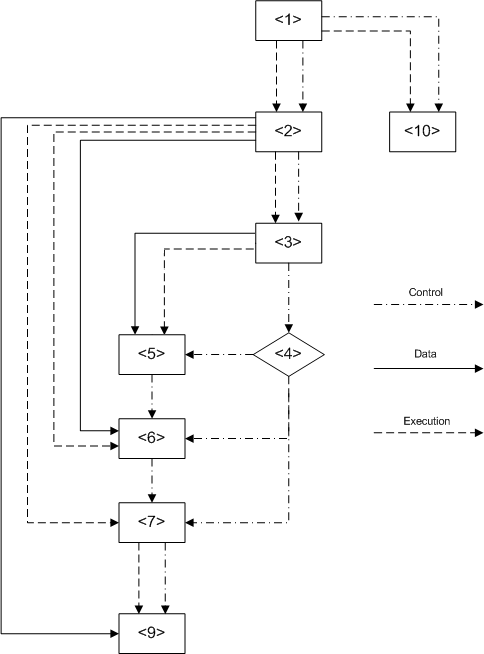
\includegraphics[scale=0.55]{Figures/exist-alg/pdg-example.png}\\[0.1cm]
  \caption[Example of program dependency graph derived from java code]{Program Dependency Graph derived from Java source code}
  \label{fig:pdg-ex}
\end{figure}

Labels attached to the nodes mean the lines where their elements located in the source code. The node labeled $<1>$ is the enter node of the PDG graph. This example example demonstrates data dependencies between nodes using variables. Node $<2>$ has initialization of text variable \texttt{text}, this variable is used in lines 6 and 7, therefore there are edges from node $<2>$ to nodes $<6>$ and $<7>$ respectfully. The dashed line from $<2>$ to $<6>$ and $<7>$ indicates that some methods on this variable used. Moreover the node $<6>$ has data edge because of input parameter of method \texttt{compareTo()}. The loop $<4>$ keeps under execution all actions inside.\\
The algorithm for clone detection offered from \cite{pdg} is based on Komondoor's Method\cite{Komondoor}:
\begin{enumerate}
  \item All nodes are hashed according to their content, similar as in AST tree compare \ref{sec: tree_tech}. Nodes with the same hash value are considered as equivalent class. The hashing process is independent from name of variables, thus only syntactically identical program elements have the same hash value. 
  \item The second step the pair of root nodes of all equivalence classes is identified. In other words roots $(r_{1}, r_{2})$ of similar sub-graphs are explored. If the predecessors $(p_{1}, p_{2})$ have the same hash value, the \textbf{slicing operation} is executed and the predecessors are added into list of pair of slices. 
  There are some cases when these pairs are not added in the list:
  \begin{enumerate}
	  \item Predecessors $(p_{1}, p_{2})$ have different hash values
	  \item Predecessors $(p_{1}, p_{2})$ have the same hash value but $p_{1}(p_{2})$ already in the slice list $r_{1}(r_{2})$. This technique provides an avoiding of endless loop.
	  \item Predecessors $(p_{1}, p_{2})$ have the same hash value but $p_{1}(p_{2})$ already in the slice list $p_{2}(p_{1})$. This technique ensures to prevent two slices from sharing the same node.
	\end{enumerate}
	\item If a clone pair of statements $(s_{1}, s_{2})$ is subsumed to another clone pair $(s_{1}', s_{2}')$ such that the following intersection takes place $s_{1} \subseteq s_{1}' \cap s_{2} \subseteq s_{2}'$. This intersection  is removed from the set of detected clone pairs. This removal must not affect on application logic since these clone pairs are not useful.
	\item The clone set is created from clone pairs as union of clone pairs. For example $(s_{2}, s_{4})$ and $(s_{2}, s_{5})$ generate a set $(s_{2}, s_{4}, s_{5})$.
\end{enumerate}

A program slicing is the union or association of the set of programs statements, that affects the values at some point of interest, referred to as a slicing criterion. Initially it is used for debugging purposes to trace the whole process of concrete data structure. This procedure is used 
in the algorithms described above in step 2. The example reveals slicing operation under function \texttt{mySlice()}:
\begin{lstlisting}
public void mySlice(){
		boolean detected = false;
		int amount = 0;
		String listOfClones = null;
		while(amount < 10){
			amount ++;
			listOfClones += "clone number: " + amount; 
		}
		System.out.println(listOfClones);
		System.out.println(amount);
	}
\end{lstlisting}
The criterion of slicing is variable \texttt{listOfClones} and therefore the new sliced instance is code:
\begin{lstlisting}
public void mySlice(){
		int amount = 0;
		String listOfClones = null;
		while(amount < 10){
			amount ++;
			listOfClones += "clone number: " + amount; 
		}
		System.out.println(listOfClones);
	}
\end{lstlisting}

The algorithm was offered by Komondoor \cite{Komondoor} in his research "Semantics-preserving procedure extraction". The noticeable feature of this whole technique is that the clones in code are searched in the one code fragment itself. This technique of clone detection based on program dependency graphs offered by Yoshiki Higo \cite{pdg} is mainly directed to find clones in the input code of course depending of programming language. Thus, there is no second input code chunk can be compared. The idea is code redundancy and optimization of execution in relative large projects when the pasted code is incorrectly changed or forgotten to be changed.
\\
The appreciable privilege of such kind of graphs is obvious. The logical relationship among variables and methods are established in the graph that makes possible to comprehend the information flow control and usability of statements. Unlike the previous ways to find clone like text-to-text \ref{sec: text_tech} or AST trees \ref{sec: tree_tech} methods are not able to keep statements of elements of statements that are not consecutively located on the source code. However it can be improved with AST tree comparison when same statements are split with regards to their locations in section Text Comparison improvement with AST trees \ref{cha:text-improvement}.
\\
There are some weaknesses of existing PDG based detection methods. Compared to other detection techniques, the first weakness is that PDG-based detection has lower performance for the detection of contiguous code clones \cite{pdg}. This is because consecutive program elements in the source code do not have necessarily data dependency or control dependency. On the other hand, line- or token-based detection methods do not consider such dependencies but rather compare program elements textually, so that these methods are productive at detecting contiguous code clones. 
Secondly the PDG-based detection has a high computational complexity. The number of nodes used as slice point is significantly large and every slice performed operation is a non-trivial task. Since the similar sub-graph needs to be identified it entails NP-complete problem because graph isomorphism is NP-complete problem.

%-----------------------------------------------------
% 3nd Chapter: Graphs comparisons algorithms
%-----------------------------------------------------
\chapter{Maximum common subtree isomorphism algorithms}
\label{cha:algorithms-to-compare}

This chapter is concerned with the issue of an important generalization of tree isomorphism, mostly known as Maximum Common Subtree Isomorphism. The goal of these algorithms is finding a largest common sub-tree between two tree structures. It plays a major role either in scientific fields or in fundamental problems. The trees can be searched for most common sub-tree from top to down, correspondingly form the head of tree till leaves, or from bottom to up, that means the search for largest sub-tree starts from leaves upwards. The algorithms are provided by Gabriel Valiente \cite{valiente}. In his book \emph{Algorithms on Trees and Graphs} he presented detailed information about Top-down Maximum Common Sub-tree and Bottom-up Maximum Common Sub-tree isomorphism. The algorithms have been implemented and adjusted to dr. Garbage tools plug-in for Eclipse integrated development environment.
\\
The sphere of application of these algorithms is mostly chemical and biological industry, however it can be applied in code comparison. Further research in this area may include not only the implementation of algorithms but also their application field. On these grounds, that the algorithms can be very helpful for tree similarity investigation. The current chapter includes an explanation of how these two algorithms have implemented in the project, about auxiliary algorithms and how they can be beneficial for the structural code comparison and similarity investigation.



\section{Top-down maximum common sub-tree isomorphism algorithm}
\label{sec:topdown}

There are two types of top-down maximum common sub-tree isomorphism algorithms. One of them finds the largest common ordered sub-tree $T$ between $ T_{1}$ and $ T_{2}$ such can found in both trees, by that when the sequence of edges from parent node does make a sense. On the contrary, the second type is the same top-down algorithm that takes into account the order of edges of parent node, during the algorithm execution. 

A top-down common sub-tree of two unordered trees $ T_{1}$ and $ T_{2 }$ is an unordered tree $T$ such that there are top-down unordered sub-tree isomorphisms of $ T$ into $ T_{1}$ and into $ T_{2}$. A maximal top down common sub-tree of two unordered  trees $ T_{1}$ and $ T_{2}$ is a top-down common sub-tree of $ T_{1}$ and $ T_{2}$ which is not a proper sub-tree of any other top-down common sub-tree of $ T_{1}$ and $ T_{2}$. A top-down of two unordered trees $ T_{1}$ and $ T_{2}$ is a top-down common sub-tree of $ T_{1}$ and $ T_{2}$ with the largest number of nodes \cite{valiente}.

\textbf{Definition 3.1}. \emph{
A \textbf{top-down common sub-tree} of an unordered tree $ T_{1} = ( V_{1}, E_{1})$ to another unordered tree $ T_{2} = ( V_{2}, E_{2})$ is a structure 
$ (X_{1}, X_{2}, M)$, where $ X_{1} = (W_{1}, S_{1})$ is a top down unordered subtree of $ T_{2}$ and $M \subseteq W_{1} \times  W_{2}$ is an ordered tree isomorphism of $ X_{1}$ to $ X_{2}$. A top-down common sub-tree $ (X_{1}, X_{1}, M)$ of $ T_{1}$ to $ T_{2}$ is \textbf{maximal} if there is no top-down common sub-tree of $ (X_{1}', X_{2}', M')$ of $ T_{1}$ to $ T_{2}$ such that $ X_{1}$  is a proper top-down common sub-tree of $ X_{1}'$ and $ X_{2}'$ is a proper top-down sub-tree of $ X_{2}'$, and it is \textbf{maximum} if there is no top-down common sub-tree $ (X_{1}', X_{2}', M')$  of $ T_{1}$ to $ T_{2}$ with the $size[X_{1}] < size[X_{1}']$\cite{valiente}.
}

%PICTURE TDMC
\begin{figure}[hb]
  \centering
  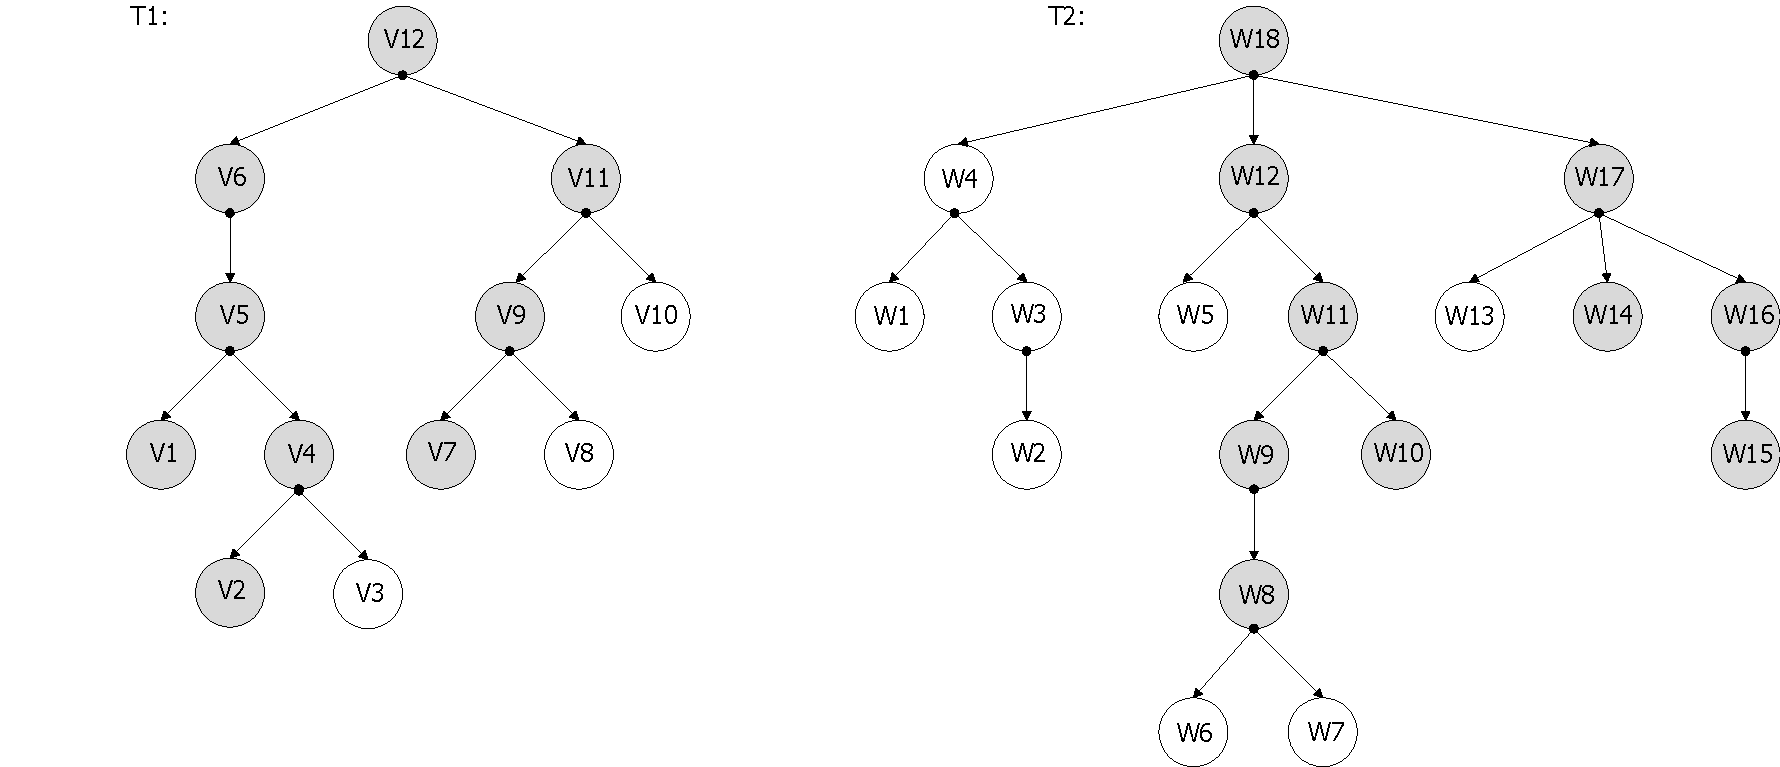
\includegraphics[scale=0.45]{Figures/algorithms/TD/top-down-max-common-example-adjusted.pdf}\\[0.1cm]
  \caption[Top-down maximum common ordered sub-tree of two unordered trees]{Top-down maximum common ordered sub-tree of two unordered trees T1 and T2. Nodes are numbered according to the order in which they are visiting during a post order traversal. The gray highlighted nodes are shaped maximum common sub-tree starting from the root \cite{valiente}.}
  \label{fig:top-down-max-common-example-adjusted}
\end{figure}

The figure \ref{fig:top-down-max-common-example-adjusted} demonstrates a partial injection $M \subseteq W_{1} \times  W_{2}$ among trees $ T_{1} = ( V_{1}, E_{1})$ and  $ T_{2} = ( V_{2}, E_{2})$ where $M  = \{ (v1,w10),  (v2,w8), (v4,w9), $ \\
$(v5,w11),  (v6,w12),  (v7,w15),  (v9,w16), $  $ (v10,w14),  (v11,w17),  (v12,w18)\}$ is unordered top-down maximum common sub-tree isomorphism $ T_{1}$ and $ T_{2 }$ \cite{valiente}.

Important to realize that the injection $M \subseteq W_{1} \times  W_{2}$ can contain different pairs of nodes, as a result there are is only one unique maximum common sub-tree available. Nevertheless the number of pairs of nodes is constant and always maximal.

If nodes $v$ is leaf $ T_{1}$ and $w$ is leaf of $T_{2 }$ accordingly mapped to each other, then the maximum common sub-tree gains size 1. Let suppose that $p$ is number of children of $ T_{1}$ and $q$ is number of children of $ T_{2}$ respectively. Consequently $ v_{1},...,v_{p}$ and $ w_{1},...,w_{q}$ are children of 
 $v$  and $w$\cite{valiente}. Solving the algorithm needs to build a bipartite graph $G=(\{v_{1},...,v_{p}, w_{1},...,w_{q} \}, E)$ on $p+q$ vertices, with edge 
$ v_{i},w_{i} \in E$  if and only if the size of maximum common sub-tree of the sub-tree $ T_{1}$ rooted at node $ v_{i}$ and the sub-tree of $T_{2 }$ rooted at node $ w_{i}$ is non zero\cite{valiente}. 
The bipartite graphs are built recursively the algorithm in one of trees $ T_{1}$ or $ T_{2}$ a leaf reaches. Let the leaf node of $ v_{i}$ of tree $ T_{1}$ is found, then a bipartite graph can be formed with node $ w_{i}$ from $ T_{2}$ at the same hierarchy level. Using the algorithm of \emph{Maximum Bipartite Weighted Matching} the corresponding parent nodes $ w_{i+1}$ and $ v_{i+1}$ gains weight one plus \emph{Maximum Bipartite Weighted Matching}(in short, MBM)of current bipartite graph.

%PIC 1
\begin{figure}
  \begin{minipage}[h]{0.60\linewidth}
    \centering
    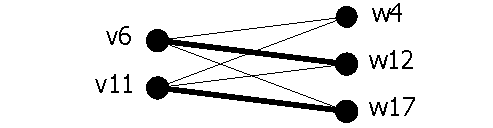
\includegraphics[scale=0.95]{Figures/algorithms/TD/1ex.pdf}\\[0.1cm]
  \end{minipage}%
  \begin{minipage}[b]{0.30\linewidth}
    \centering
\begin{tabular}{|c|c|c|c|}
\hline
    & w4 & w12                       & w17                       \\ \hline
v6  & 3  & \cellcolor[gray]{0.9} 5 & 3                         \\ \hline
v11 & 4  & 5                         & \cellcolor[gray]{0.9}4 \\ \hline
\end{tabular}
\end{minipage}
\caption[The final solution of bipartite matching]{The solution MBM of bipartite graph brings $5+4=9$ weight from previous solutions}
\label{fig:ex1}
\end{figure}
%PIC 1

%PIC 3
\begin{figure}[h]
  \begin{minipage}[h]{0.60\linewidth}
    \centering
    
\includegraphics[scale=0.95]{Figures/algorithms/TD/3ex.pdf}\\[0.1cm]
  \end{minipage}%
  \begin{minipage}[h]{0.30\linewidth}
    \centering
\begin{tabular}{|c|c|}
\hline
   & w2 \\ \hline
v1 &  \cellcolor[gray]{0.9}1  \\ \hline
v4 & 1  \\ \hline
\end{tabular}
\end{minipage}
\caption[]{The $v_{1}$ and $v_{4}$ are leaf nodes of the left branch of $ T_{1}$, and leaf node $w_{2}$ of $ T_{2}$. The edge $(v_{1},v_{4})$ is selected with \emph{MBM} algorithm. }
\label{fig:ex3}
\end{figure}
%PIC 3

%PIC 2
\begin{figure}
  \begin{minipage}[h]{0.60\linewidth}
    \centering
    
\includegraphics[scale=0.95]{Figures/algorithms/TD/2ex.pdf}\\[0.1cm]
  \end{minipage}%
  \begin{minipage}[b]{0.30\linewidth}
    \centering
\begin{tabular}{|c|c|c|}
\hline
   & w1 & w3                        \\ \hline
v5 & 1  & \cellcolor[gray]{0.9} 2 \\ \hline
\end{tabular}
\end{minipage}
\caption[]{The edge $(v_{5},v_{3})$ gains weight equal to two from previous solution \ref{fig:ex3}, due to the parent node}
\label{fig:ex2}
\end{figure}
%PIC 2

As an example can be taken from figure \ref{fig:ex1}. As said, the nodes are being traversed until leaf node in the trees $ T_{1}$ or $ T_{2}$ is found. Let consider the left branch of $ T_{1}$, namely leaves $v_{1}$ and $v_{4}$ and respectively the left branch of $ T_{2}$, namely leaf $w_{2}$. A created bipartite graph is depicted at figure  \ref{fig:ex3}. The corresponding table shows weights of edges. Since these two are leaves they equal one. With algorithms \emph{MBM} the edge $v_{1}$ and $w_{2}$ is being selected. Once the selection is done, the algorithm take their parent nodes, accordingly $v_{5}$, $w_{3}$ and $v_{3}$. The appropriate bipartite graph is constructed. The edges  $v_{5}$ and $w_{3}$ have weight equal to one initially in table \ref{fig:ex2}, but since from previous solution \ref{fig:ex3}  the node $v_{1}$ has a parent $v_{5}$, the edge $(v_{5},w_{3})$ gets weight equal to two. Likewise the edge  $(v_{6},w_{4})$ in table \ref{fig:ex1} has a value three based on previous result.

By the same way all entries in table \ref{fig:ex1} have been built. Passing through the tree $ T_{1}$ at another left branch until leaves $v_{2}$ and $w_{3}$ the similar bipartite graph can be formed \ref{fig:ex6}. As said before, the current edges get same weight equal to one. The edge $(v_{2},w_{8})$ is selected regards the \emph{MBM} algorithm. Under those circumstances the next bipartite graph can be built \ref{fig:ex5}. Based on previous solution the edge $(v_{4},w_{9})$ obtains weight equal to two.

%PIC 6
\begin{figure}[h]
  \begin{minipage}[h]{0.60\linewidth}
    \centering
    
\includegraphics[scale=0.95]{Figures/algorithms/TD/6ex.pdf}\\[0.1cm]
  \end{minipage}%
  \begin{minipage}[b]{0.30\linewidth}
    \centering
\begin{tabular}{|c|c|}
\hline
   & w8 \\ \hline
v2 & \cellcolor[gray]{0.9} 1  \\ \hline
v3 & 1  \\ \hline
\end{tabular}
\end{minipage}
\caption[]{Starting from leaves select of both trees select edges with maximum weight. According to the algorithm the connection $(v_{2},w_{8})$ has been selected.}
\label{fig:ex6}
\end{figure}
%PIC 6

%PIC 5
\begin{figure}[h]
  \begin{minipage}[h]{0.60\linewidth}
    \centering
    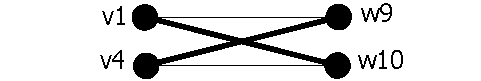
\includegraphics[scale=0.95]{Figures/algorithms/TD/5ex.pdf}\\[0.1cm]
    
  \end{minipage}%
  \begin{minipage}[b]{0.30\linewidth}
    \centering
\begin{tabular}{|c|c|c|}
\hline
   & w9 & w10 \\ \hline
v1 & 1  & \cellcolor[gray]{0.9} 1   \\ \hline
v4 &  \cellcolor[gray]{0.9}2  & 1   \\ \hline
\end{tabular}
\end{minipage}
\caption[]{Since previous decision was $(v_{2},w_{8})$, and they respectively are parents of $(v_{4},w_{9})$ its weight of edge gains one plus the decision equal to one.}
\label{fig:ex5}
\end{figure}
%PIC 5

%PIC 4
\begin{figure}[h]
  \begin{minipage}[h]{0.60\linewidth}
    \centering
    
\includegraphics[scale=0.95]{Figures/algorithms/TD/4ex.pdf}\\[0.1cm]
    
  \end{minipage}%
  \begin{minipage}[b]{0.30\linewidth}
    \centering
\begin{tabular}{|c|c|c|}
\hline
   & w5 & w11 \\ \hline
v5 & 1  &  \cellcolor[gray]{0.9} 4   \\ \hline
\end{tabular}
\end{minipage}
\caption[]{The the sum maximum matched edges from \ref{fig:ex5} equal to 3, in the same manner the edge $(v_{5},w_{11})$ gains 3 + 1 = 4 weight}
\label{fig:ex4}
\end{figure}
%PIC 4

Having a look at table in \ref{fig:ex1} in cell $(v_{6},w_{12})$ where the value is 5. This has been formed due to the solution from table \ref{fig:ex4}, because nodes $(v_{6},w_{12})$ are direct parents of $(v_{5},w_{11})$. likewise all other leaves in both trees are investigated and on-fly the tables with weight are filled out. The table in \ref{fig:ex1} is completed by the same way as described above. At the end the maximum bipartite weighted matching algorithm selects the edges $(v_{6},w_{12})$ and $(v_{11},w_{17})$ because they bring the maximum weight of the bipartite graph. In this case two branches in \ref{fig:top-down-max-common-example-adjusted} are picked and the corresponding nodes are grey highlighted forming the maximum common sub-tree from the bottom.\\
Description of the operating principle of algorithm is represented  below:

\begin{lstlisting}
list<node, node> topDownMaxCommonSubtreeIsomorphism(const TREE T1, const TREE T2){
node r1 = root(T1);
node r2 = root(T2);
traverse(node r1, node r2);
M = list<node, node>
reconstruct(r1, M);
}
\end{lstlisting}

This method traverses recursively simultaneously through T1 and T2 till leaves of them are founded.
\begin{lstlisting}
void traverse(node v, node w){
int p = v.getNumberOfChildren();
int q = w.getNumberOfChildren();
if(p == 0 or q == 0) return 1;

Array matrix = new Array[p][q];

for(i = 0; i < p; i++){
	for(j = 0; j < q; j++){
		node vChild = v.getChild();	
		node wChild = w.getChild();
		matrix[i][j] = <vChild, wChild, -1>
	}
}

int res = 1;
if(p != 0 and q != 0){
bipartiteGraph bg = createBipartiteGraphFromMatrixEntry(matrix);
if (bg.numberOfEdges == 0) return 0;

list<edge> L = MaxWeightedBipartiteMatching(bg);
forall(e, L){
result += e.getCounter();
}
matching(list<edge> L);
return res;
}
}
\end{lstlisting}
This method reconstructs the TDMC unordered sub-tree isomorphism mapping.
\begin{lstlisting}
reconstruct(node r1, list<node, node> M){
M[r1] = r2;
list<node> L;
preorder-tree-traversal(L, T1);
forall(node v, L){
	forall(node w, B[v]){
	if(M[T1.parent(v)] == T1.parent(w)){
		M[v] = w;
		break;	
	}
}
}
\end{lstlisting}

Puts into list B matched edges for further reconstruction
\begin{lstlisting}
matching(list<edge> L){
	forall(e, L){
	B[r1].insert(r2);
	}
}
\end{lstlisting}

In order to define the largest subtree the algorithm uses an auxiliary Maximum Weight Bipartite Matching sub-algorithm. The Maximum Weight Bipartite Matching implements remarkable \textbf{Hungarian Method} that promotes to find edges in a weighted bipartite graph so that the sum of the weights in the matching has a maximal value. The Hungarian Method solves the assignment problem and uses a modified shortest path search in the augmenting path algorithm. These two algorithms have been implemented in dr. Garbage algorithms libraries.

Overall, this complex algorithm is useful tool to find an abstract similarity between tree structures. Application fields can be very various: chemistry, biology, computer vision and pattern recognition.

\section{Bottom-up maximum common sub-tree isomorphism algorithm }
\label{sec:bottomup}

There are two types of bottom-up maximum common sub-tree isomorphism algorithms. One of them finds the largest common ordered sub-tree $T$ between $ T_{1}$ and $ T_{2}$ such can found in both trees, by that when the sequence of edges from parent node does make a sense. On the contrary, the second type is the same top-down algorithm that takes into account the order of edges of parent node, during the algorithm execution. 

A bottom-up common sub-tree of two unordered trees $ T_{1}$ and $ T_{2 }$ is an unordered tree $T$ such that there are top-down unordered sub-tree isomorphisms of $ T$ into $ T_{1}$ and into $ T_{2}$. A maximal bottom-up common sub-tree of two unordered  trees $ T_{1}$ and $ T_{2}$ is a bottom-up common sub-tree of $ T_{1}$ and $ T_{2}$ which is not a proper sub-tree of any other bottom-up common sub-tree of $ T_{1}$ and $ T_{2}$. A bottom-up of two unordered trees $ T_{1}$ and $ T_{2}$ is a bottom-up common sub-tree of $ T_{1}$ and $ T_{2}$ with the largest number of nodes \cite{valiente}.

\textbf{Definition 3.1}. \emph{
A \textbf{bottom-up common sub-tree} of an unordered tree $ T_{1} = ( V_{1}, E_{1})$ to another unordered tree $ T_{2} = ( V_{2}, E_{2})$ is a structure 
$ (X_{1}, X_{2}, M)$, where $ X_{1} = (W_{1}, S_{1})$ is a bottom-up unordered subtree of $ T_{2}$ and $M \subseteq W_{1} \times  W_{2}$ is an ordered tree isomorphism of $ X_{1}$ to $ X_{2}$. A bottom-up common sub-tree $ (X_{1}, X_{1}, M)$ of $ T_{1}$ to $ T_{2}$ is \textbf{maximal} if there is no bottom-up common sub-tree of $ (X_{1}', X_{2}', M')$ of $ T_{1}$ to $ T_{2}$ such that $ X_{1}$  is a proper bottom-up common sub-tree of $ X_{1}'$ and $ X_{2}'$ is a proper bottom-up sub-tree of $ X_{2}'$, and it is \textbf{maximum} if there is no bottom-up common sub-tree $ (X_{1}', X_{2}', M')$  of $ T_{1}$ to $ T_{2}$ with the $size[X_{1}] < size[X_{1}']$\cite{valiente}.
}

%PICTURE OF BUMC
\begin{figure}[th]
  \centering
  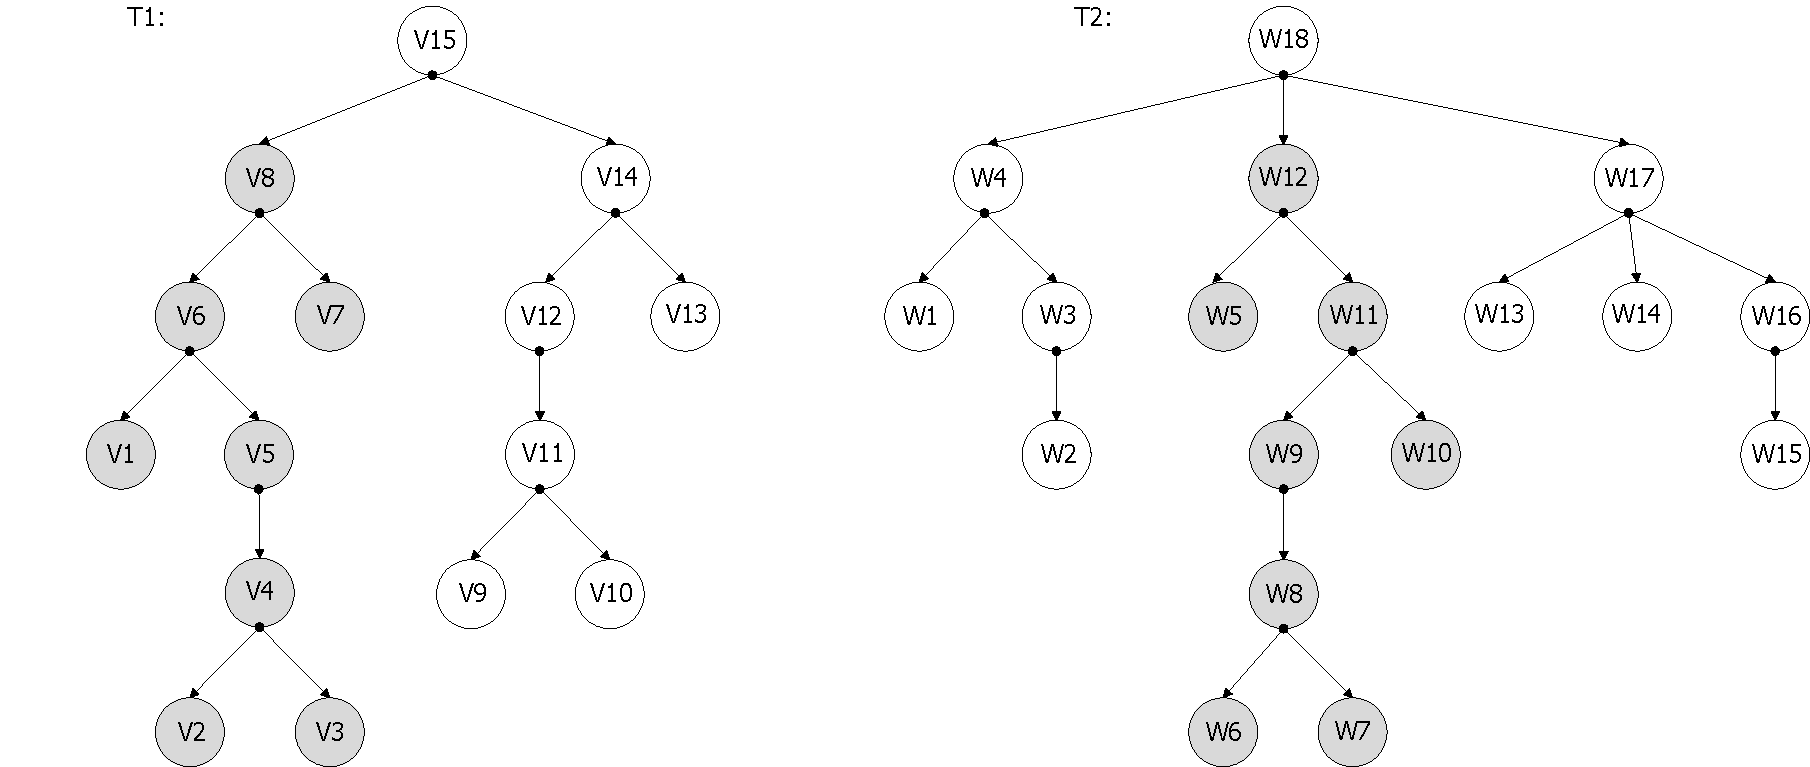
\includegraphics[scale=0.45]{Figures/algorithms/BU/bottom-up-max-common-example.pdf}\\[0.1cm]
  \caption[Bottom up maximum common sub-tree of two unordered trees]{Bottom Up maximum common ordered sub-tree of two unordered trees T1 and T2. Nodes are numbered according to the order in which they are visiting during a post order traversal. The gray highlighted nodes are shaped maximum common sub-tree starting from the leaves \cite{valiente}.}
  \label{fig:bottom-up-max-common-example}
\end{figure}

The figure \ref{fig:bottom-up-max-common-example} demonstrates a partial injection $M \subseteq W_{1} \times  W_{2}$ among trees $ T_{1} = ( V_{1}, E_{1})$ and  $ T_{2} = ( V_{2}, E_{2})$ where $M  = \{ (v1,w10),  (v2,w6), (v3,w7), $ \\
$(v4,w8),  (v5,w9),  (v6,w11),  (v7,w5), $  $ (v8,w12)\}$ is unordered bottom-up maximum common sub-tree isomorphism $ T_{1}$ and $ T_{2 }$ \cite{valiente}.

The problem of finding a maximum common sub-tree isomorphism between two trees $ T_{1}$ and $ T_{2 }$, where $ T_{1}$ has $n_{1}$ nodes and $ T_{2}$ has $n_{2}$ respectively can be reduced to the problem of partitioning $ V_{1}\bigcup V_{2}$ into equivalent classes of bottom-up sub-tree isomorphism. Two nodes are equivalent if and only if the bottom-up unordered sub-tree rooted at them are isomorphic.

\begin{figure}[h]
  \centering
  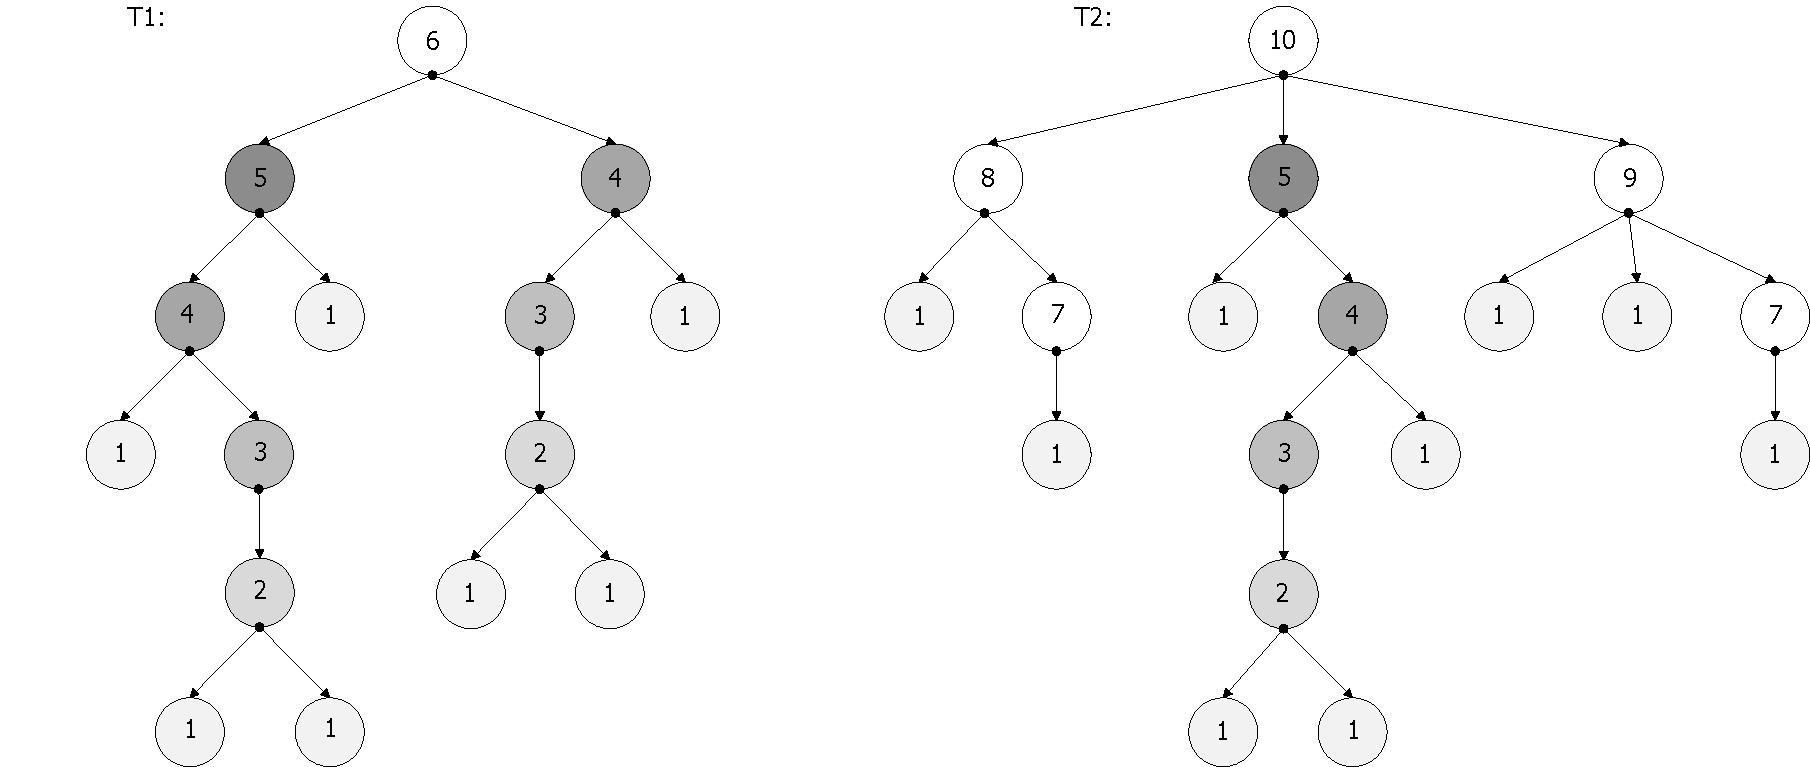
\includegraphics[scale=0.45]{Figures/algorithms/BU/bottom-up-max-common-example-equivalence.pdf}\\[0.1cm]
  \caption[Bottom up unordered sub-tree isomorphism equivalence classes on trees] { Bottom-up maximum common equivalence classes reflected to the figure \ref{fig:bottom-up-max-common-example}. The node are numbered according to the equivalence class to which they belong and the equivalence classes are shown highlighted in the different shades of gray\cite{valiente}.}
  \label{fig:bottom-up-max-common-example-equivalence}
\end{figure}

The algorithm start with a partition a tree into bottom-up equivalence classes.
Let the number of known equivalence classes be initially equal to 1, corresponding to the equivalence class of all leaves in the trees. For all nodes v of $ T_{1}$ and $ T_{2 }$ in post-order, set the equivalence class of $V$ to 1 if node $v$ is a leaf. Otherwise, look up in the dictionary the ordered list of equivalent classes to which the children of node $v$ belong. If the ordered list (key) is found in the dictionary then set the equivalence class off node $v$ to the value (element) found. Otherwise, increment by one the number of known equivalence classes, insert the ordered list together with the number of known equivalence classes in the dictionary, and set the equivalence class of node $v$ to the number of known equivalence classes.

In general this complex algorithm is useful tool to find an abstract similarity between tree structures from leaves. Application fields are beneficial in areas like chemistry, biology, computer vision and pattern recognition. 


%-----------------------------------------------------
% 4th Chapter: Code compare experiments
%-----------------------------------------------------

\chapter{Experimental analysis between structural and textual methods}
\label{cha:experimental}
\section{Introduction in experiments}

This chapter is dedicated to comprehend the methods of textual and structural compare approach. As a result of the experimental analysis an improved concept of structural approach compare  is created. For the better understanding of probable improvements of code comparison using existing algorithms, some possible ideas of implementation and an amount of experiments is required. In order to build a proper tool, or at least a concept, in Eclipse plug-ins at Dr. Garbage some hand experiments in code should be fulfilled. 
\\
There are many combination how code can be smartly changed, then existing methods of compare sometimes are not able to identify code plagiarism.  All these test cases are performed in Eclipse IDE \cite{eclipse_site} and divided into sections where mostly text component of is changed which sometimes does not influence on the application logic. It assist to figure out why textual comparison is insufficient of careful code investigation. There are two the most well-known methods how to build a graph from source code with dr. Garbage Eclipse plug-ins. These analysis steps are fulfilled in this chapter:
\begin{enumerate}
  \item Research on Flowchart graphs derived from java source code, using existing methods for maximum common tree isomorphism from chapter \ref{cha:algorithms-to-compare} and embedded Eclipse compare editor:	
  
  \item Research on abstract syntax tree derived from java source code, using existing methods for maximum common tree isomorphism from chapter \ref{cha:algorithms-to-compare} and embedded Eclipse compare editor:	
  
  \item Research on java byte code comparison using graph theory.
\end{enumerate}

All test sets are investigated under java methods and functions, in other words two functions with similar application logic. In some cases, the demonstrative result of comparison is not important, but the statistical data are substantial. The analysis phase is carried out under small snippets of code, thereby the real difference, application logic and code similarity, is observed in details by the experimenter. 
\\
Playing around with the patterns of code changing variables, names, sequences of commands, adding loops or conditions and apply on it methods of textual comparison. This comparison is already implemented in Eclipse IDE \cite{eclipse_site}, with so-called command "compare with each other by member" that calls text compare editor. This type of comparison provides a pop-up window, where two pieces of code are compared, particularly line by line.
\\
In parallel, a control flowchart graphs or AST trees from the functions are being created and compared using implemented algorithms top-down maximum common and bottom-up maximum common(in short, TDMC and BUMC). The further task is to figure out the difference/similarity from graphical visual comparison. Consequently these both results must be matched and recorded for succeeding research. Take into account that textual compare is guided to investigate precise difference in code, whereas TDMC and BUMC are concerned to find out tree isomorphism, in particular similarity. Statements of code are nodes in compared trees depends on tree organization. When two fragments of code are compared, text editor highlights an amount statements and amount of isomorphic nodes are highlighted in trees. This can be computed into real figures and quantitative compared to see which can identify the distinction. Statements can be a name of variable, sequence of commands or assignment of variable. It completely depends on tree organization. For example, \texttt{if(people.count() > = 10)} for the flowchart it represents one a decision node, rhombus formed and consequence branches depend on condition itself. The same chunk of code in AST represents a branch with root node the while expression and sub branches, for instance \texttt{people} and \texttt{10}.
\\
Let the set $S_{1}$ is all statements marked (found mismatches) in text compare editor and the set $S_{2}$ is amount of all mismatched nodes after the algorithm execution.
The derived results from experiments can be as listed: 
\begin{enumerate}
  \item Text compare and TDMC/BUMC find the same differences $S_{1} = S_{2} $. Thus, textual found statement are not equal to their according non-isomorphic nodes.
  \item Text compare and TDMC/BUMC deliver similar difference $S_{1} \cap S_{2} \neq \varnothing $. It means in some cases the algorithms are able to detect same mismatches and sometimes not.
  \item Text compare and TDMC/BUMC provide full difference $S_{1} \cap S_{2} = \varnothing $, consequently the intersection of all marked statements is an empty set.
\end{enumerate}


% JAVA SOURCE CODE EXPERIMENTS
\section{Experiments on Java source code flowcharts}

A flowchart is a type of diagram that represents an algorithm, work-flow or process, showing the steps as boxes of various kinds, and their order by connecting them with arrows. This diagrammatic representation illustrates a solution model to a given problem. Flowcharts are used in analyzing, designing, documenting or managing a process or program in various field s\cite{wiki_flowchart}.

Dr. Garbage tools \cite{drgarbage} provides a solution how to represent sequential flowchart alongside to Java source code (see figure \ref{fig:java-flowchart-example}).
\begin{figure}[h]
  \centering
  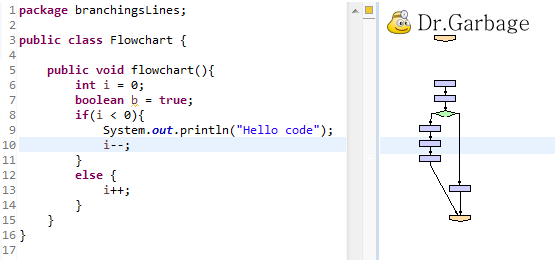
\includegraphics[scale = 0.65]{Figures/Java-flowchart-exp/java-flowchart-example.png}\\[0.1cm]
  \caption[Java flowchart diagram opened in java source-code visualizer]{Example of source code visualizer}
  \label{fig:java-flowchart-example}
\end{figure}

A depicted flowchart can be easily extracted into control flow graph. For another similar function, it can be transformed into next control flow graph. Afterwards these two graphs are being compared using existing TDMC[\ref{sec:topdown}] and BUMC[\ref{sec:bottomup}] algorithms. 

\begin{figure}[h]
  \centering
  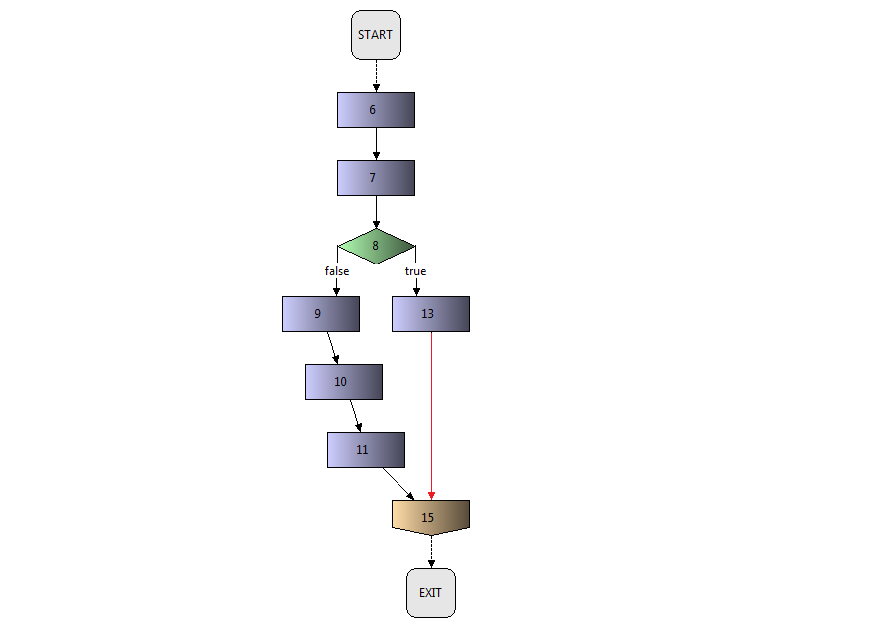
\includegraphics[scale = 0.5]{Figures/Java-flowchart-exp/control-flow-graph.png}\\[0.1cm]
  \caption[Extracted control flow graph from java source code]{Extracted control flow graph from Java source code. The red arrow is removed according to Spanning Tree Algorithm in order to build a tree structure with minimal losses of edges. The number inside of node is number of global string in text.}
  \label{fig:control-flow-graph}
\end{figure}

Unfortunately, these two algorithms are applicable only for tree data structures. For this reason, this problem can be reduced, removing minimum number of edges to get a spanning tree. Thus, the edges in the input graphs are reduced by Spanning Tree Algorithm with minimal losses. The removed edges are red highlighted, hence this for this structure TDMC and BUMC algorithms[\ref{cha:algorithms-to-compare}] can be easily applied.

To conduct an experiments a sequence of actions and issued statistics are needed. After conducted experiments, taking into account the derived statistic, an outgoing conclusion takes place. The steps to analyze approach bringing better result are carried through sequence of actions:
\begin{itemize}
	\item Writing of two similar java functions in Eclipse IDE.
	\item Applying for them text-to-text comparison with Eclipse IDE compare editor.
	\item Declaration of the statistic, respectively how many statements are different.
	\item Creation of a source-code flowchart diagram for both functions.
	\item Apply TDMC and BUMC algorithms to get structural difference.
	\item Receiving of statistical overview, respectively how many nodes have been  mapped as the result of deviation or similarity.
\end{itemize}

In this section all experiments have been executed by hand using plug-in tool Graph Comparison in Eclipse from dr. Garbage project. Before get started, a several rules how to evaluate code difference in text and in graph must be established. It is one of the crucial moment, because followed data statistic are used in further tool development. For the estimation of structural difference there are criterias listed:
\begin{enumerate}
	\item Each java statement is considered as one simple node in extracted flowchart.
	\item Percentage of difference in textual compare is computed, thereafter it roughly equals to division of number of marked to unmarked statements. The same procedure of average similarity proportion is calculated after tree comparison. Since there are two algorithms looking for isomorphic nodes, the statistic is taken from the most suitable one, which specially brings the largest number of matched nodes.
\end{enumerate}

Mostly all calculations are performed roughly, because there are many criterias how to evaluate the logic and structure difference. Nonetheless, from this perspective these rules are enough to examine graph's similarity and make a conclusions.

For the text difference found via Eclipse compare editor tool a criterias to evaluate similarity are complied:
\begin{itemize}
	\item Percentage is computed by maximum number of found mismatched strings to the maximum number of string of compared objects.
	\item If in one string of code only one symbol has been covered as found, then the difference is calculated as a division of one to amount of symbols in this line. This assists to get statistical data precisely.
\end{itemize}

\begin{figure}[h]
  \centering
  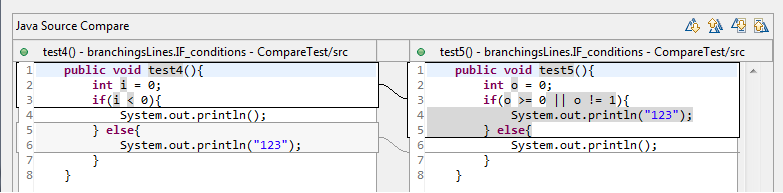
\includegraphics[scale = 0.5]{Figures/Java-flowchart-exp/example-graph.png}\\[0.1cm]
  \caption[Two pieces of code are compared with Eclipse text compare editor]{Two pieces of code are being compared with Eclipse Text Comparison}
  \label{fig:example-graph}
\end{figure}

And after generation of two graphs, these both are compared(see the figure \ref{fig:graphs-compared}) using existing TDMC and BUMC[\ref{cha:algorithms-to-compare}] algorithms.
\begin{figure}
  \centering
  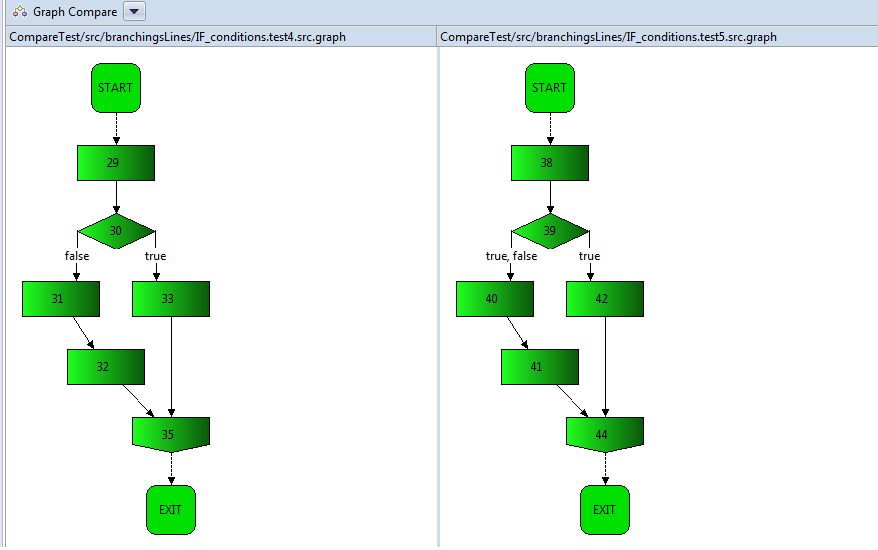
\includegraphics[scale = 0.6]{Figures/Java-flowchart-exp/graphs-compared.png}\\[0.1cm]
  \caption[Compared flowchart graphs using TDMC algorithm ]{Compared source code flowcharts graphs using Top down maximum common sub-tree algorithm \ref{sec:topdown}. The compare is done only after removing back edges.}
  \label{fig:graphs-compared}
\end{figure}


\begin{table}[h]
\begin{tabular}{|c|c|c|c|c|}
\hline
\multicolumn{3}{|c|}{Compare experiments}                & Text -to-text compared     & Graph compared              \\ \hline
Test id & Name of functions & \begin{tabular}[c]{@{}c@{}}Real  code \\ difference \%\end{tabular} & \begin{tabular}[c]{@{}c@{}}Layout difference\\  \% found\end{tabular} & TDMC\&BUMC similarity \% found \\ \hline
1       & t1() and t2() &             50             &             100               &               100             \\ \hline
2       & t1() and t3() &               50           &                   100         &            75                \\ \hline
3       & t1() and t4() &                50          &             100               &              100              \\ \hline
4       & t1() and t2() &                50          &        100                    &                80            \\ \hline
5       & t1() and t5() &                50          &            100                &            100                \\ \hline
6       & t6() and t7() &               33           &                33            &               100             \\ \hline
7       & ti1() and ti2() &              10            &                100            &             0               \\ \hline
8       & ti2() and ti3() &             16             &                100            &              100              \\ \hline
9       & ti3() and ti4() &               25           &         100                   &                 66           \\ \hline
10      & ti4() and ti5() &                 50         &           100                 &                   0         \\ \hline
11      & ti6() and ti7() &                 90         &           100                 &                   42         \\ \hline
\multicolumn{3}{|c|}{Overall results:}                & 93.9 \%  &  69\% \\ \hline

\end{tabular}
\caption[Experimental results between textual and structural comparison on flowcharts]{The table demonstrates results of java-source comparison using text-to-text compare method and application of algorithms to their flowchart diagrams.}
\label{table:tests-table}
\end{table}

The table \ref{table:tests-table} shows results of java source code experiments. Existing algorithms [\ref{cha:algorithms-to-compare}] and Eclipse text-to-text comparison have been used to reveal the best approach of code comparison. As it said above, the difference code can be figured out either structurally or simple text comparison. Based on results in the table \ref{table:tests-table} the apparent conclusion are composed:
\begin{itemize}
	\item If the application logic is totally different (For example the condition \\ \textbf{if(people.count() $>$ 10)}) then Eclipse compare editor finds the difference, thus condition itself is highlighted. The graphical comparison with  TDMC\&BUMC  is not able to see this distinction. It is obvious, since graph theory in this case is able to find how similar structure of code fragments. The conducted example \ref{fig:graphs-compared} above can testify this conclusion. In this way, graph theory is not applicable to differentiate logic of application.
	
	\item In opposite said above, the graphical compare is quite useful tool to investigate a code structure. For example, if another third party person has changed local variables, the structure remains same, thus TDMC\& BUMC (especially TDMC) find high level of similarity. This approach is enough to build a new concept allowing to investigate the code similarity more precisely. 
	
	\item The graph is totally bound to lines of codes. If one brace is shifted, then it is considered one more block in the flowchart graph (Dr. Garbage Source Code Visualizer \cite{drgarbage} generates extra node for each code operator). Hence, TDMC is not able to find following branch where there an extra node and generated Java source code graph is not optimized for comparison.
	
	\item Text-to-text compare is enough to investigate a text difference because this tool finds every different sub-string in code line. But as stated above, changing variables, sequence of operators or even production same loops with different operators the text-to-text compare find too much unmatched strings. Eventually, the result of text compare looks like a disorder with same and unmatched sub-strings.  	

\end{itemize}

% JAVA AST TREE CODE EXPERIMENTS
\section{Experiments using Abstract Syntax Tree graphs}

In this section the abstract syntax trees are generated from java source code are used to be compared. In contrast to the flowcharts, the AST trees do not contain cycles, therefore it is not necessary to remove any back edges to get a tree structures. The most notable advantage of AST trees creation is inflexible structure and proper ordered depths nesting of vertices according to the code. For example, a loop in code has a number of sub-statements as parent-child relation, the same way the nesting of branch is organized.

% Please add the following required packages to your document preamble:
% \usepackage[table,xcdraw]{xcolor}
% If you use beamer only pass "xcolor=table" option, i.e. \documentclass[xcolor=table]{beamer}
\begin{table}[h]

\begin{tabular}{|p{0.5cm}|p{3cm}|p{2cm}|p{3cm}|p{5cm}|}
\hline
\rowcolor[HTML]{C0C0C0} 
Test id & Case of mismatch                                           & Text difference                  & Structural difference                           & Result \\ \hline
1       & redundant statement added                      & found                            & found                                    & both techniques are able to notice the difference visually \\ \hline
2       & decision statement changed                     & found                            & not found but structure is same delivered & text compare highlights changed condition   \\ \hline
3       & statements have been swapped                   & found but is incorrect presented & found                                    & swapped statements can be easily identified \\ \hline
4       & decision statement changed;\newline parameters changed & found                            & not found but structure is same delivered                                & structure of code is absolute identical\\ \hline
5       & names of variables changed                     & found                            & not found                                &                                             structure of code is absolute identical, i.e. 100\% code similarity \\ \hline
\end{tabular}
\caption[Summary of comparison between textual and structural compare with AST]{Results showing the difference of comparison between combination of AST trees and existing algorithms and traditional textual compare }
\label{table:ast_res}
\end{table}

The table \ref{table:ast_res} demonstrates intermediary results between structural and textual comparison. Primarily, can be said that the sub-tree algorithms are very suitable to define similarity if code fragments have a complementary structure. Thus, the text compare is beneficial tool to identify precise difference in:
\begin{enumerate}
	\item Small code fragments, for the reason that large compare results bring quite complicated view.
	\item Code fragments with very similar code construction, where there are insignificant changes, for instance conditions in decision statement, or another style of increment writing.
\end{enumerate}
After analysis part on AST trees and applied algorithms, the next assertions can be expressed:
\begin{enumerate}
	\item The algorithms are supportive to identify the percentage of plagiarism/similarity.
	\item Applicable for large pieces of code, on condition that statistical details required. Specifically, assuming that, it is necessary to know how alike compared objects.
\end{enumerate}
Overall, AST trees have their own profits of comparison in contrast to text-based approach. 
Based on these outcomes, some improvements for the structural comparison are described in this work. Particularly, the technique that allows to built more similar AST trees whereas the different style of programming performing same application logic. The chapter \textbf{Techniques to normalize AST improving structural comparison} \ref{cha:ast_normal} reports the actual solution. In addition, the chapter \textbf{Text comparison improvement with AST trees} \ref{cha:text-improvement} discloses another approach of code text representation.

% JAVA BYTE CODE EXPERIMENTS
\section{Experiments on JavaByte Code}
\label{sec: java-code-experiments}

In this section an investigation regards java byte-code comparison is expound. Unlike Java source code, the corresponding byte code has practically no application logic. In spite of this the topic must be researched for the clone detection. \\
Citation from the IBM \textbf{developerWorks} journal, "Understanding bytecode and what bytecode is likely to be generated by a Java compiler helps the Java programmer in the same way that knowledge of assembly helps the C or C++ programmer" \cite{ibm}. 

\begin{figure}[h]
  \centering
  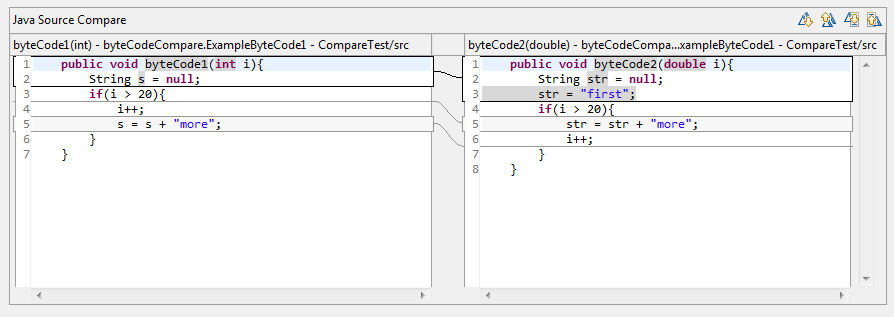
\includegraphics[scale = 0.55]{Figures/bytecode-compare/example-of-bytecode-text-compared}\\[0.1cm]
  \caption[Java byte code compared in Eclipse text compare editor]{Java byte code compared using compare editor in Eclipse environment}
  \label{fig:example-of-bytecode-text-compared}
\end{figure}

Assignment of variable in java byte code includes java byte code address and according type suffix/prefix. The complexity of java byte code compare with graph theory is that the code has no structured logic like java source code. However, there are some clues hot to find some code clones between two java compiled files. In this case, the comparison must be performed within one complied .class file, not a methods as it described above in java source code.

\begin{figure}[h]
  \centering
  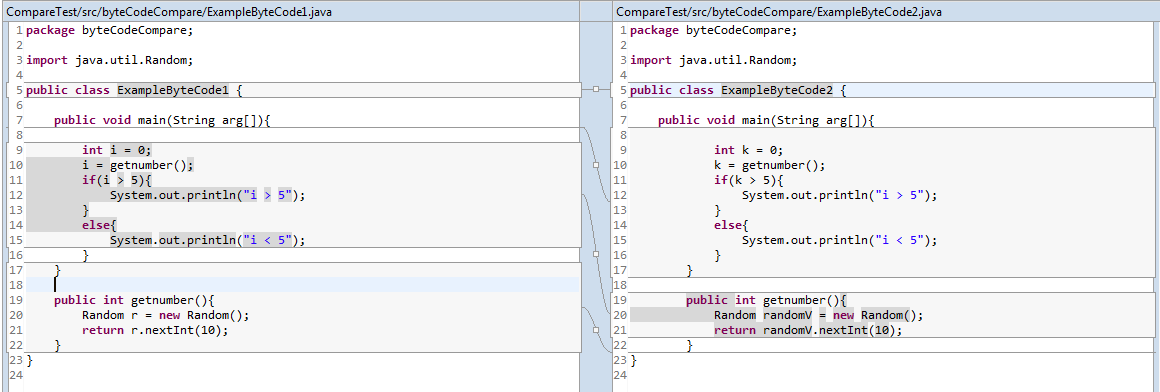
\includegraphics[scale = 0.4]{Figures/bytecode-compare/example-of-bytecode-original-compared}\\[0.1cm]
  \caption[Java byte code compared with text Eclipse compare editor]{Java byte code compared with text Eclipse compare editor.}
  \label{fig:example-of-bytecode-original-compared}
\end{figure}

To detect clones or find similarity between two complied java function using graph creation is not suitable technique for this. It may be an idea to create a bipartite graph, where partition $A$ is all nodes with corresponding instructions and partition $B$ is formed by the same way. The relations among the node are a Cartesian product. Then, an algorithm that searches for same instructions that exist in both partitions. This task, can be organized with collection and theory of sets.
\begin{lstlisting}
        /* L14 */
        0 bipush 15;
        2 istore_1;               /* people */
        /* L15 */
        3 getstatic 19;           /* java.lang.System.out */
        6 ldc 25;                 /* "jf" */
        8 invokevirtual 27;       /* void println(java.lang.String s) */
        /* L16 */
        11 iload_1;               /* people */
        12 invokestatic 33;       /* java.lang.String java.lang.Integer.toString(int s) */
        15 astore_2;              /* s */
        /* L17 */
        16 return;
\end{lstlisting}

Assignment of variables can be found with association of opcodes, for example: \texttt{aload\_0} or \texttt{istore\_2}. 
This is relation to the type of the data that the instruction operates. The prefix $a$ means that the opcode is manipulating an object reference and the prefix $i$ means the opcode is manipulating an integer. 
The list $ L_{1}$ represents the first collection of instructions from code $a$, and $L_{2}$ has instruction from code $b$. 
Same the instructions can be found in the parsing of both lists.
If element $E_{i}$ contains \texttt{istore\_1}, then the same list $L_{1}$ is searched for any instructions operate with $\#1$ index. This reminds a slicing operation described in chapter \textbf{Existing comparison methods for plagiarism detection}, section PDG-techniques \ref{sec: pdg_tech}. Dr. Garbage plug-ins tool allows to built flowchart graphs that have data-flow and vertex content holds java byte code information, however it is now sufficient to define code clone with such types of tree. Firstly, this is a graph, therefore the isomorphism costs are very expensive. Secondly, a trivial addition of statement into flowchart increases the nesting of flowchart, that is complicated for the clone search.
All these instructions with index $1$ are encompassed into set $S_{i}$. The maximum intersection set $S_{i}'$ of instructions is searched in the list $L_{2}$ that have same index, that bijection function $f$ exists that $f: S_{i} \rightarrow S_{i}'$. In other words, a subset with maximum number of instruction in $L_{1}$ is searched, that similar to $S_{i}$.

%-----------------------------------------------------
% 5th Chapter: Graph transformation algorithms
%-----------------------------------------------------


%\chapter{Tree transformation algorithms}
%\label{cha:graph-transformation}
%
%This chapter describes 

\chapter{Techniques to normalize AST improving structural comparison}
\label{cha:ast_normal}
\section{Code similarity issues}
Researches show that many massive development projects have a duplicated code, which is generally result of copying and pasting existing pieces of code. Moreover, the code can be completely redone, changing name of variables, in some cases replace lines of code. Nevertheless, the most sophisticated part comes when a same command can be in the code substituted. It is known, that from programming perspectives, for instance, a loop can be differently created, however application logic stays unchanged. For instance, there three fundamental ways to reproduce the iteration statements, namely: \emph{pre - condition}, \emph{post - conditions} and so-called \emph{for-loop}. The function can be reworked by so delicate way, that none of any text-to-text compare finds similarity. Mostly, only controversy of both fragments in compare editor will be displayed.
However, the functions bring the same application logic. This code clones can be found almost everywhere, especially in free-published software, the most notable example is clone pair between FreeBSD and Linux, that code listing \ref{listing1} presents. 

The following example \ref{listing1} depicts that the functions used in open-source operation systems Linux and FreeBSD are similar and have same application logic. On the occasion that these functions are compared with text compare, then definitely one line with increment of variable \texttt{frameGroupLine} is highlighted. 
\newpage
\begin{lstlisting}[caption={Clone pair between FreeBSD and Linux}, label = listing1, numbers=left, numbersep=-5pt]
	public void fragment1(){
			int frameGroupLine = 10;
			for(int Cnt = 1; Cnt < frameGroupLine;  Cnt =+ 2)
			{
				if(Cnt*4 != 2){
					frameGroupLine++;
				}
			}
		}
			
	public void fragment2(){
			int frameTeamLine = 10;
			for(int Counter = 1; Counter < frameTeamLine;  Counter =+ 2)
			{
				if(Counter*4 != 2){ 
					frameTeamLine = frameTeamLine + 1;
					}
			}
		}	
\end{lstlisting}


In the chapter Existing comparison methods for plagiarism detection \ref{cha:methods}, namely in token-based technique there are some pre-processes to prepare input string for optimized graph creation. Therefore, the Sub-tree suffix algorithm \ref{sec: tocken_tech} is able to bring better results.
For example, Karp-Rabin fingerprints algorithm reviewed in \cite{software_clone_detection} is used for calculating the fingerprints of all
length $n$ sub-strings of a text. First, a text-to-text transformation is performed on the considered source for discarding the uninterested characters.

Afterwards, the entire text
is subdivided to a set of sub-strings so that every character of the text appears in at least
one substring \cite{software_clone_detection}. After that the matching sub-strings are identified. 

In that stage, a further transformation is applied on the raw matches to obtain better results. Instead of applying
a set of text transformations, he applies several different transformation scenarios
from a combination of basic transformations such as for identifying near-miss duplication he
attempted to find a normalized/transformed text by removing all white space characters
except line separators and by replacing each maximal sequence of alphanumeric characters
with a single letter \texttt{i}. For example, a line \texttt{for(k = 1; k <= n; k + +) \{ } is replaced by
the line \texttt{i(i = i; i < =; i++)}. This kind of transformation gives too more false positives. But, this idea can be used in structural similarity comparison. Since the TDMC algorithm \ref{sec:topdown} looks the largest sub-tree, it means the largest sub-tree is kind of common part of two derived AST trees from code fragments. \\

\section{Tree restructuration methods}
Consider the line number 16 from the listing \ref{listing1}. If this line \texttt{frameGroupLine = frameGroupLine + 1;} will be converted into one format of sub-tree, that indicates the same as \texttt{frameGroupLine++;}. As the result, this another way created sub-tree can be found with TDMC or BUMC algorithms. Consequently it brings more covered nodes that signalize more similarity, exactly that improves the statistic of covered nodes.

\begin{lstlisting}[caption= {Normalized function \texttt{normalizedFragment()} concerning variable \texttt {frameGroupLine}}, label = listing2, numbers=left, numbersep=-5pt]
	public void normalizedFragment(){
		int frameGroupLine = 10;
		for(int Counter = 1; Counter < frameGroupLine;  Counter =+ 2)
		{
			if(Counter*4 != 2){ 
				frameTeamLine++;
			}
		}
	}
\end{lstlisting}

In the function \texttt{fragment2()} one the increment of variable \texttt{frameTeamLine} is differently written. From text-to-text compare the functions are different at this point. If the text code similarity will be calculated as mismatch in this place, then these two fragments are not same (probably $90\%$ similarity). Using Abstract Syntax Trees Optimization, this types of structure can be converted in the same sub-tree of whole AST tree. Thereby, these two different text structures are represented as same sub-tree. 

\vspace{4mm}

\begin{figure}[h]
  \centering
  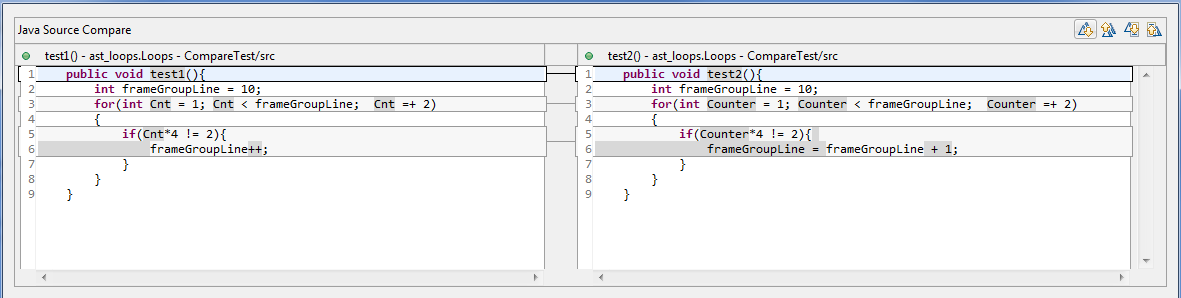
\includegraphics[width=1.00\textwidth]{Figures/AST-optimization/text-to-text-compare.png}\\[0.1cm]
  \caption[Example shows that text compare is not able to identify similarity]{Example shows that text compare editor is not able to identify exact similarity. The presented chunk of code is relatively small and facilitates to see clone visually for user. Though for large code fragments the user cannot say unambiguously that there is clone in the code. }
  \label{fig:text-to-text-compare}
\end{figure}

On figure \ref{fig:text-to-text-compare} the example demonstrates how these two functions are compared using Eclipse Text comparison window. After creation and comparison these two AST trees, it can be easily seen that sub-trees (the increment) are different.

\begin{figure}[h]
  \centering
  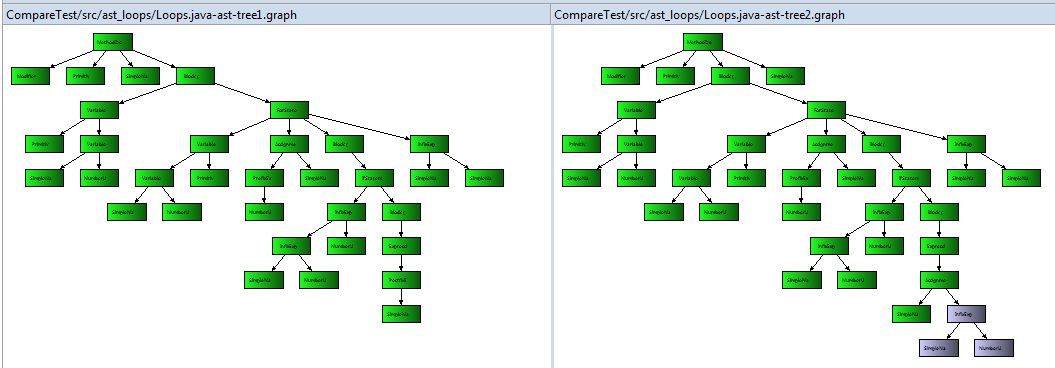
\includegraphics[width=1.00\textwidth]{Figures/AST-optimization/tree-compared1}\\[0.1cm]
  \caption[Graph comparison on similar AST trees using TDMC algorithm]{Graph comparison of function fragment1() and fragment1() using TDMC algorithm \ref{sec:topdown}}
  \label{fig:ast-graph-compare-similar-tdmc}
\end{figure}

From the figure \ref{fig:ast-graph-compare-similar-tdmc} TDMC algorithm finds incomplete code similarity since not all nodes have been covered. From statistical point of view using simple math, the percentage of similarity is figured out: 37 nodes in the \texttt{test2()} and 3 of them are not covered. Thus, the calculation indicates  $\left ( 1 - \left (\frac{3}{37} \right ) \right )\cdot 100 = 91\%$ code similarity according to AST trees and applied TDMC algorithm.

This mismatch can be optimized during AST tree production. These two lines of code \texttt{frameGroupLine++;} and \texttt{frameGroupLine = frameGroupLine + 1;}
must be built as a same sub-tree, accordingly same structure and same number of nodes. Using this simple replacement it allows to built a similar AST trees, when logic is same but the source code text is different. Consequently the converted AST trees to some extent are independent from source code and can be compared to explicit the difference.

The example described above is relatively small, but exact showing how this logic can be circumvented. Also in pre-processing of AST tree can be included all possible java operators. This process called code normalization, and can be prepared before the AST tree will have been built. \\

\begin{table}[h]
\centering 
\begin{tabular}{|l|l|l|}
\hline
     Operator                        & input   & output     \\ \hline
\multirow{2}{*}{postfix}     & \texttt{i++}     & \texttt{i = i + 1  }  \\ \cline{2-3} 
                             & \texttt{i--}     & \texttt{i = i - 1  }  \\ \hline
\multirow{2}{*}{prefix}      & \texttt{++i}     & \texttt{i = i + 1 }   \\ \cline{2-3} 
                             & \texttt{--i }    & \texttt{i = i - 1}    \\ \hline
\multirow{7}{*}{assignments} & \texttt{i *= n } & \texttt{i = i * n } \\ \cline{2-3} 
                             & \texttt{i /= n  }& \texttt{i = i / n } \\ \cline{2-3} 
                             & \texttt{i \%= n }& \texttt{i = i \% n }\\ \cline{2-3} 
                             & \texttt{i -= n } & \texttt{i = i - n } \\ \cline{2-3} 
                             & \texttt{i += n  }& \texttt{i = i + n } \\ \cline{2-3} 
                             & \texttt{i =+ n } & \texttt{i = i + n}  \\ \cline{2-3} 
                             & \texttt{i =- n } & \texttt{i = i - n } \\ \hline
\end{tabular}
\caption[Combinations of statement substitutions to create more similar trees]{The table demonstrates a proper string transformation for AST tree optimization. In event of occurrence  of input operator, the original can be substituted before AST tree have been built.}
\label{table:operators}
\end{table}

The table \ref{table:operators} presents possible java string transformation depending on the input command. Thus the fragment of code will be better prepared for AST tree reformation. The trees of both both comparing functions will more similar that TDMC algorithm finds more similarity. Using statistical data to consider how function similar to each other the formula can be derived. Let $NC$ is subset all of unmatched nodes then\\
$ N \subseteq T_{1}: n \in NC $ and $ M \subseteq T_{2}: m \in NC $ \\
The trees are combined as set of vertexes and edges, thereby $T_{1} = (V_{1}, E_{1})$ and $T_{2} = (V_{2}, E_{2})$ respectfully, the the probability that two functions have same structure takes place: \\
\begin{gather*}
similarity(\%) =  \left ( 1 - \left (\frac{max(|N|, |M|)}{max(|V_{1}|, |V_{2}|)} \right ) \right )\cdot 100 
\end{gather*} \\
where $|V_{1}|$ and $|V_{2}|$ are cardinalities of their subsets. In other words the formula can be described as ratio of maximum number of unmatched nodes between $T_{1}$ and $T_{2}$ to maximum number of nodes in both trees $T_{1}$ and $T_{2}$. 

Overall, such combination of tree normalization and applied maximum sub-tree algorithms has an initial stage of the structural comparison. The beneficial point is an additional parser, that restructures AST tree according to some rules. It allows to get more precise statistical results. The further development in this field can be dedicated to an extension of existing regulations. Particularity, loop implementation or restructure of tree among \texttt{switch} and \texttt{if} statements, that implemented as same control flow with different commands. 


\chapter{Text comparison improvement with AST trees}
\label{cha:text-improvement}

In the chapter described about existing comparison methods, section section text based techniques \ref{sec: text_tech} is written about disadvantages of text-to-text compare, namely changing the sequence of statements which do not influence on application logic. However in this case, comparison of text-to-text is sensitive  and thereby its representation of difference is redundant.

\section{Problems related to text editor representation}
This example \ref{fig:text-to-text-compare-shifted} demonstrates how text compare is not available to notice the string difference in case some statements have been simply replaced. Namely the operators: \texttt{case 0:} and \texttt{case 4:} from figure \ref{fig:text-to-text-compare-shifted} have been replaced but text compare find this difference. 
\begin{figure}[h]
  \centering
  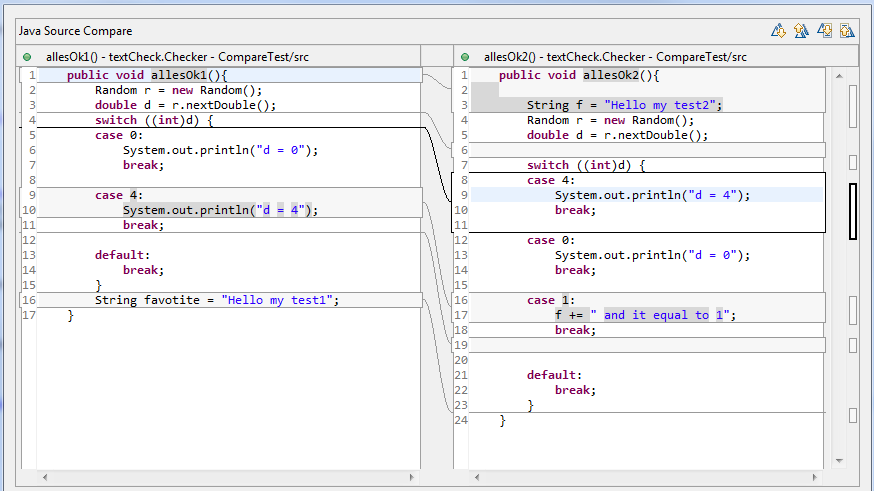
\includegraphics[scale = 0.5]{Figures/text-to-text/text-compare-shifted.png}\\[0.1cm]
  \caption[Textual comparison example showing inability to detect swapped clones]{Textual comparison example showing inability to detect swapped clones in java source code.}
  \label{fig:text-to-text-compare-shifted}
\end{figure}



Moreover, when this code mostly changed, namely the names of variables, line position in code, thereby not impacting on the application logic of function then it is much more difficult to clarify the code difference. Thus, comparing two function using text-to-text compare, it can be that the final result is totally mixed, however these functions are almost identical. Comparing of relatively large code fragments which are consecutively swapped according to time line makes text-to-text comparison not so much effective, especially on the back code compare representation. The inefficiency consists in complexity of imposed comparison, in some cases it is not readable. 

Why text-to-text cannot find these obvious differences? This algorithm for string search is described in chapter \ref{sec: text_tech}. Using the Suffix sub-tree algorithm,  according to research of Roy, Chanchal Kumar \cite{software_clone_detection}, there are some disadvantages that can interpret the issue described above on picture \ref{fig:text-to-text-compare-shifted} where some sub-strings are not found described in following citation:
\begin{quote} 
This tools does not support exploration and navigation through the duplicated code. Detection accuracy is low e.g., cannot detect code clones written in different coding styles. For example "\{" position of if-statement or while-statement. Cannot detect code clones using different variable names, e.g. to identify the same logic code as code clones even if variable names are different\cite{software_clone_detection}. 
\end{quote}

Hypothesized that the Suffix sub-tree algorithm is more negatively related to proper code compare in case if clone detection is being searched. This can be improved with help of tree based algorithms techniques;
\begin{figure}[h]
  \centering
  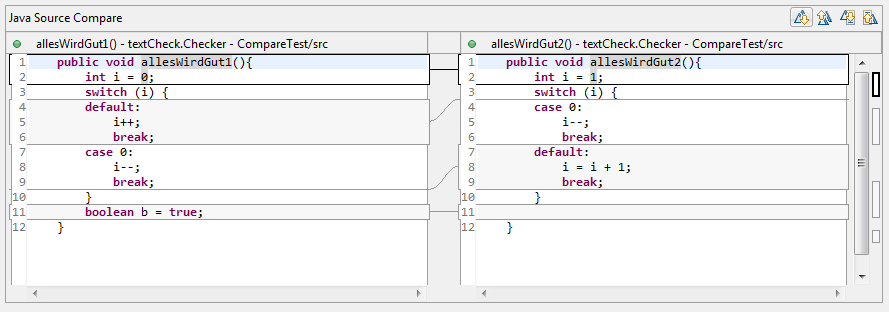
\includegraphics[width=1.00\textwidth]{Figures/text-to-text/text-compared-for-improve}\\[0.1cm]
  \caption[Text comparison example where strings of code are replaced.]{Example of text-to-text demonstrating the code difference using the Suffix sub-tree algorithm }
  \label{fig:text-compared-for-improve}
\end{figure}

As prerequisites take the following example depicted on the picture \ref{fig:text-compared-for-improve}. Considering the example very carefully, line by line, it is easy to get an idea how these two peaces of code are organized. In the line \#2, the obvious mismatch variable \texttt{i = 1} to compared with \texttt{i = 0} and \texttt{false} to \texttt{true} are gray highlighted in the third line.
\\
Up next, comes the \texttt{if} operator, where there are two and three blocks respectfully. They make almost the same logic however the sequence of statements is changed.
The last difference on the line \#11: the function \texttt{test2()} contains extra command \texttt{b = true;}.
At the end of function \texttt{test2()} there is an additional operator. Notice that, the example is relatively small and has not some much different commands and operators and moreover, when sequence of statements is shifted, swapped or changed. It can be that two functions are so complex modificated, thereby the text compare yields a mix of various lines. 

\section{Algorithm using AST trees}
To improve this code similarity search, a code can be transformed into Abstract Syntax Tree (in short, AST) and both tree are traversed synchronously checking matched nodes. The biggest advantage of methods based on trees that AST trees are built independently of sequence of commands. The difference in this trees is unordered range of nodes. It means that these AST trees are taken into consideration as unordered trees, where ordering is not specified for the children of each vertex. Swapped statements can be limited by one block, in other words the higher rank command represents a parent-node and within this block there swapped sub-command that are 
descendant-nodes. The sequence of descendant-nodes is arbitrary, since AST trees are also built as unordered.\\
\begin{figure}[h]
  \centering
  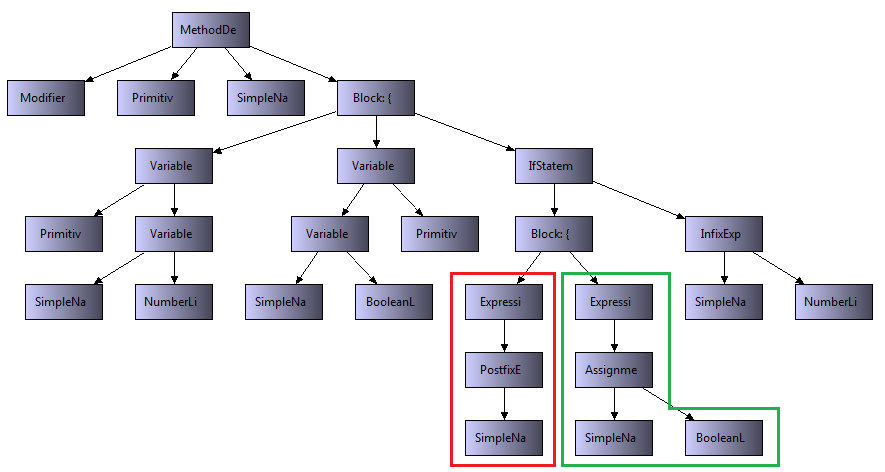
\includegraphics[width=1.00\textwidth]{Figures/text-to-text/graph-compared1.png}\\[0.1cm]
  \caption[Abstract Syntax Tree with colored clone frames]{Abstract Syntax Tree of function \texttt{test1()} with colored clone frames .}
  \label{fig:graph-compared1}
\end{figure}

\begin{figure}[h]
  \centering
  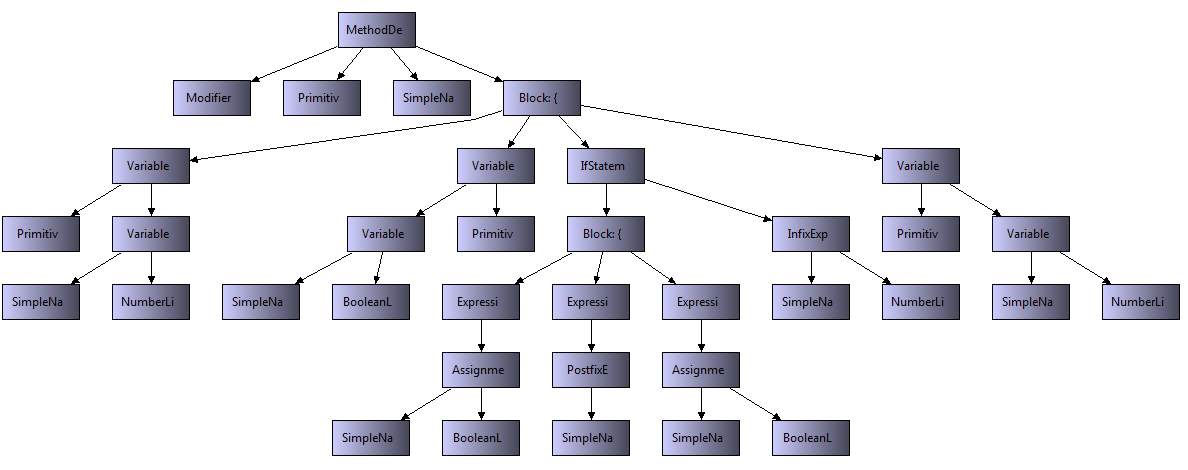
\includegraphics[width=1.00\textwidth]{Figures/text-to-text/graph-compared2.png}\\[0.1cm]
  \caption[]{Abstract Syntax Tree of function \texttt{test2()} with colored frames indicating similarity and redundancy.}
  \label{fig:graph-compared2}
\end{figure}

Example \ref{fig:text-compared-for-improve} and derived AST trees \ref{fig:graph-compared1} and  \ref{fig:graph-compared2} indicates similarity, difference and redundancy:
\begin{enumerate}
  \item Red and green framed branches are equal in figures \ref{fig:graph-compared1} and \ref{fig:graph-compared2}: \texttt{i++} and \texttt{b = false }, therefore the nodes in this branch must be marked as \emph{matched}, in other words the same without structural difference. 
  
  \item The yellow frame marks out the statement \texttt{b = true;} line, that is redundant in \texttt{test1()} in this branch, specifically in \texttt{if(i > 1)\{ } condition. Hence, only this statement must be highlighted in text compare windows as \emph{mismatched}. 
  
  \item The blue frame in picture \ref{fig:graph-compared2} denotes a new command line, namely \texttt{double d = 1.1;}. This statement is also redundant and comes from another nesting level and must be marked as possible mismatch. In Cartesian product this parent node is not matched, hence the whole branch starting from the parent is marked as \emph{mismatched}.

\end{enumerate}

The picture \ref{fig:graph-compared1} shows how AST tree from function \texttt{test1()} is being built from the source code. As said above, the presented AST tree \ref{fig:graph-compared1} is unordered, thus the replaced lines of code and the nested operators and independent from each other. The trees traversal enables to identify the concrete difference in source code, independent how the code is organized. The evident mismatch must be referred to the source code. The idea is to keep the current command or statement in the AST tree node, i.e. to keep inside a meta-information: a current text position of command or statement in the corresponding node. 

These coloured framed branches are visible and signalize a discrepancy between two AST trees. Apparently that, the same discrepancy makes sense to be proper delivered into text editor,  specifically into text-to-text comparator. For this reason a modified traversal algorithm is required. The Breadth-first search traverse algorithm is performed on two AST trees derived from $test1()$ and $test2()$ methods. At same node depth $i$-level a Cartesian Product from one parent-node among nodes is built (a bipartite graph, almost identical strategy has been used in existed algorithm TDMC \ref{sec:topdown})to search for different, missed or redundant nodes and mark them accordingly for further text representation. However, in this bipartite graph the content is compared. For the algorithm optimization technique all descendant-nodes, respectfully branch and its content is being hashed. This procedure is done during AST tree creation. 
\\
Taking all sketches into consideration  the following algorithms steps can be derived:
\begin{enumerate}
  \item AST tree creation from the source code. This AST tree is unlike to original because of content of nodes. This node meta-information is extended and recorded during tree forming. Each node keeps the following information:
  	\begin{enumerate}[label*=\arabic*.]
		\item Content - exact statement, operator or command in text format. For example: \texttt{if (i != 1)}  	 
		\item Hashed value sub-branch - during the tree creation each sub-tree content is hashed. For example, the root node of statement:
\begin{lstlisting}[frame = none]
	if (i != 1){
	 i = i + 1;
 	}
\end{lstlisting}
		 has a for-example MD5 hash-value of \texttt{i = i + 1;}\\ that equals to \texttt{05b200b7f0b9b4bdf3f4a1b1d8aa041c}. This allows to decrease the complexity of algorithm to search sub-strings. If large sub-functions are same, comparing their hash-values gains a lot of performance. In the best case the complexity can be $O(1)$, instead of searching out all sub-nodes.
		 \item Global text positions - precisely the number of line of the node element and start and end point coordinates within this line. It needs for the proper text difference representation on text-compare window.
		 \item A variable \emph{matched} that keeps information about whether this statement exists in both functions and must not be highlighted.
		 \item Any other meta-information for statistical data to be extended.
  	 \end{enumerate}
  \item Once AST tree is built, the Bread-first search (in short, BFS) is applied on the trees. The traverse is executed simultaneously comparing $i$-nested level of each tree. Firstly the content of nodes is compared, once the content is matched textually, up next the hashed-values are compared. Since hashed value are unique identifiers there are two scenarios:
	  \begin{enumerate}[label*=\arabic*.]
  			\item Hash-values are same - in this case the whole branch is marked as \emph{matched}. It says that on this nested level there are same statement in both compared statements.
  			\item Hash-values of  entries are different - the BFS is being continued further and step 2. is repeated to investigate the leaves where difference is placed since the hash-values are not matched.
	  \end{enumerate}
  \item Once BFS is finished the procedure to deliver result back to text is started. This is second traversal that runs over all unmatched nodes and distributes difference on the compared text. Nodes not marked as \emph{matched} are represent the code redundancy. In most cases, the highlighted elements are explicit redundant with regards of executed comparison, in other words the compare fragments have not exact same highlighted statements.
\end{enumerate}
\begin{figure}[th]
  \centering
  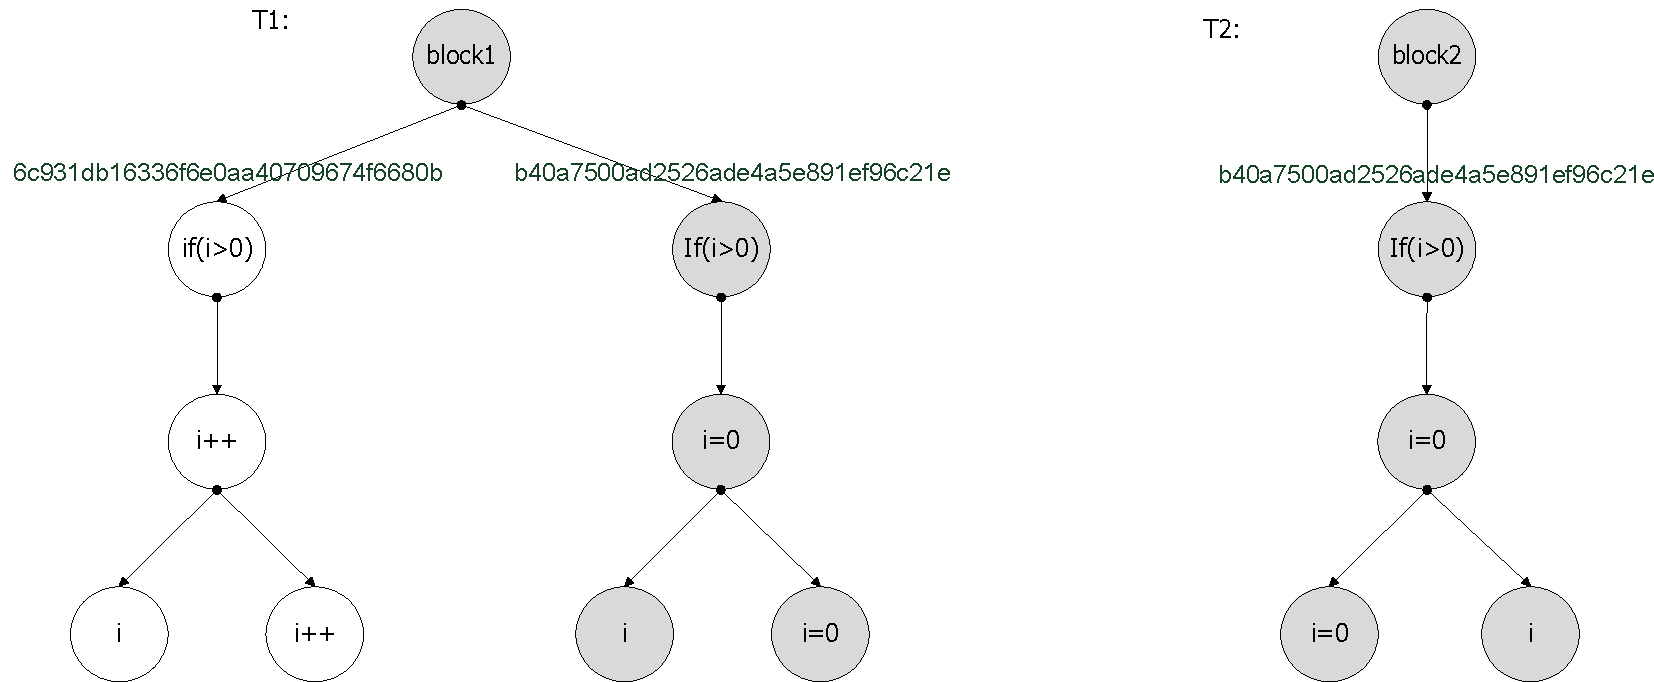
\includegraphics[scale = 0.5]{Figures/text-to-text/example-of-text-opt.pdf}\\[0.1cm]
  \caption[Example of hashed branch content to optimize the search algorithm]{Example of hashed branch content that assists to optimize the algorithm search for clones. The more similar compared fragments of the faster the algorithms execution.}
  \label{fig:example-of-text-opt}
\end{figure}

The figure \ref{fig:example-of-text-opt} shows two AST tree compared during tree-traversal. Firstly, the content of $2$-nested level is compared and both have
\texttt{if(i > 0)} that indicated that nodes are same. In the described second step of the algorithm the hash-values containing the whole content of sub-tree are compared. The left branch of $T_{1}$ is unique to the main branch $T_{2}$ and consequently these both are marked \emph{matched}. Obviously a question appears, why firstly not to compare by the hash-value since it is unique, avoiding compare of the content. It does not make a sense because the parent-node has content with sub-elements and the difference is takes place there. The algorithm seeks out for a concrete mismatch, and there is no sense to stop the BFS in hash-values are different whereas content is same. To be precised, the difference is placed in the descendant-nodes that must further investigated.

\section{Conclusion and gathered statistics}
The complexity of algorithms in the worst case can be $O(3\cdot|V|)$, where $V$ number of created AST nodes, and three traversal are required: creation of the tree, search for clones and representation in text compare window. The hashing technique simplifies the complexity roughly 20\% since large computer systems have duplicated code.

Disadvantages of this approach are restriction of the search space. The AST tree represents a non-flexible data structure which does not depend on real logic of application as it described about Program Dependency Graphs \ref{sec: pdg_tech}. The sequence of statements is limited by one parent node located on $i$-nested level. It can be possible when there is the same block of code statements where the duplicated fragment is placed $i+1$-nested, i.e. under another code operator. Nevertheless, the application logic  of code fragment is not different. Further research must be dedicated to above described problem. The idea can be taken from PDG-methods \ref{sec: pdg_tech}. To trace the variables or to slice under required condition are basics to detect clones located in different branches.

Statistical data interpretation is a crucial moment after fragments have been compared. The statistics can interpret in the first row how similar were the code fragments. \\
\begin{gather*}
similarity(\%) =  \left ( 1 - \left (\frac{max(|T_{1}'|, |T_{2}'|)}{max(|T_{1}|, |T_{2}|)} \right ) \right )\cdot 100 
\end{gather*} \\
Where: $T_{1}' \subseteq $\{all mismatched nodes in $T_{1}$ \} and \\$T_{2}' \subseteq $\{all mismatched nodes in $T_{2}$ \}
\\
The statistical data play a big role in code similarity investigation. After execution of comparison a collection of derived figures must be provided:
\begin{itemize}
	\item Statistical review of changed command structures. Particularly, this is information shows proportion of \texttt{if}-conditions have been changed for instance. In additional, a command statements structure redundancy, for example quantity of extra \texttt{for} loop in both compared code chunks.
	\item Code redundancy - in other words how much code redundancy in both code fragments.
\end{itemize}
Overall, the idea how find similar or same disordered pieces of code with AST tree is quite argumentative. At least, using AST is improvement of standard the Suffix-tree based algorithm, that compares line by line not taking into consideration the application logic. On the one hand, text-to-tex comparison is is useful to detect swapped statements, despite the fact that the logic of application is not disturbed. 
However, conceding that the similar code has another small changes, like names of variables or various index increments statements, then text-compare provides rather sophisticated and hard read results. The result of the algorithms is highlighting in text only such elements, that both redundant in compared objects, of course with following statistic

On the other hand, granted that this sensitive is code difference is really necessary, it is reasonable to use standard text comparison. Assuming the fact, that this sensitive approach is needed, i.e. exchanged statements must be identified, the compromise decision in further research  may be a usage of different colors of highlighting.

%-----------------------------------------------------
% 5th Chapter: Conclusion
%-----------------------------------------------------


\chapter{Conclusion}
\label{cha:Conclusion}

The discussions regards plagiarism detection and successive avoiding and maintenance of it are not a innovation today. However nowadays, in software maintenance this theme is object of current interest. As said in the introduction, the real code development process can not go without reusable code, that is not pragmatical in usage. It implies that misuse of copying-pasting of existing code fragments is common situation in the development process. In length of time, the code handling becomes progressively harder, because of software clones. Another problem is comparison code fractions for similarity. There is a necessarily when fragments of code need to be compared to figure out precisely and visually where this difference come from. 
Sometimes, when code fragments are too large to seek out each difference a statistical data representation is sufficient proof whether codes are similar or different with probability.
\\
The process analysis phases in chapter Experimental analysis between structural and textual methods of code comparison reports about ways of comparison using tree-based approach and in addition these techniques are compared with textual method. In this process, the existing two algorithms, namely Top-down and Bottom-up maximum common sub-tree isomorphism have been involved to define a a structural similarity. It turns out, that the larger common sub-tree, in most cases sub-tree found from top to down, more similar their code structures. From this experience has been derived that AST trees are more suitable to compare code for similarity and also partly to investigate exact difference.
\\
Furthermore the existing well-know techniques of clone detection and compare have been mentioned. From experimental part it is become known that text-based approach is insufficient to detect precise difference in code. This is justified by the fact that code has its own logic, and changing text textual components of it, the logic stays same. Nonetheless, textual does not provide sufficient facts that code implements same logic, as result that is code plagiarism. 
Clear code text is non-flexible structure for text-based algorithms, therefore the text-to-text compare methods have an independent gap between logic and text.
\\
This work describes an interpretation of algorithms which finds the largest sub-trees between input two trees taken from Gabriel Valiente \cite{valiente}. The algorithms have been implemented and adjusted to the project dr. Garbage - is a set of open source plug-ins for control flow analysis of java programs. These algorithms are useful not only in software area but in chemical and biological branches, because essences learnt there can be defined as tree structures.
\\
The chapters Techniques to normalize AST and Text comparison improvements announce an ideas to enhance quality of code search with actual method of clone detection. The first improvement report about tree optimization during it form from code, by that makes compared structured uniformed. The second is about technique to improve textual compare, including of application logic, with tree-based method.
\\
Taking everything in consideration, the overall conclusion can be formulated like: each detection technique has its own relative advantages and disadvantages, and no technique is superior to any of the other techniques in all aspects.

%-----------------------------------------------------
% Literature
%-----------------------------------------------------

\newpage
%\bibliographystyle{plain}
\begin{thebibliography}{100} % 100 is a random guess of the total number of references 
\addcontentsline{toc}{chapter}{Bibliography}
%Example:
%\bibitem{ch11} George H.L. Fletcher and Catharine M. Wyss, "Data Mapping as Search", Computer Science Department, School of Informatics, Indiana University, Bloomington, USA. 

 \bibitem{drgarbage} Sergej Alekseev, Peter Palaga and Sebastian Reschke, Tutorials of The Dr. Garbage Tools Project 2014,  URL: \url{http://www.drgarbage.com}, \\last visited: 03.11.2014

\bibitem{graph_compare} Sergej Alekseev, Adam Kajrys and Andreas Karoly \emph{ Graph theoretical algorithms for control flow graph comparison}, Proceedings of the 13th IASTED International Conference on Software Engineering, 2014
 
\bibitem{valiente} Gabriel Valiente, \emph{Algorithms on Trees and Graphs}, Springer-Verlag Berlin and Heidelberg GmbH,  December 2010.

\bibitem{wiki_flowchart} Udemy.com is a platform for on-line learning: Flowcharts,\\ URL: \url{https://www.udemy.com/blog/flowchart-examples/}, \\last visited: 25.08.2014
 
\bibitem{software_clone_detection} Roy, Chanchal Kumar; Cordy, James R. \emph{"A Survey on Software Clone Detection Research".} Technical Report No. 2007-541,  School of Computing, Queen's University, Canada, September 26, 2007.

\bibitem{graph_isomorphism_is} Koebler Johannes; Schoening, Uwe. \emph{"Graph isomorphism is low for PP",} In \emph{Journal of Computer and System Sciences} 37.3, Theoretische Informatik, Universitaet Ulm, July 1991, pp. 5-11

\bibitem{baker} Brenda S. Baker \emph{"A Program for Identifying Duplicated Code",} In \emph{Computing Science and Statistics: Proceedings of the 24th Symposium on the Interface},  AT\&T Bell Laboratories, Murray Hill, New Jersey, March 1992, pp. 49-57

\bibitem{change_distilling} Beat Fluri, Student Member IEEE; Michael Wuersch, Student Member IEEE; Martin Pinzger, Member IEEE and Harald C. Gall, Member IEEE \emph{"Change Distilling: Tree Differencing for Fine-Grained Source Code Change Extraction"}, In \emph{Software Engineering, IEEE Transactions on 33.11 }, Department of Informatics, University of Zurich, Zurich, November 2007, pp. 725-743 

\bibitem{tocken_kamiya} Toshihiro Kamiya, Member, IEEE, Shinji Kusumoto, Member, IEEE, and Katsuro Inoue, Member, IEEE \emph{"CCFinder: A Multilinguistic Token-Based Code Clone Detection System for Large Scale Source Code",} In \emph{Software Engineering, IEEE Transactions},  July 2002, pp. 654-670

\bibitem{flavius} Flavius-Mihai Lazar \emph{"Clone detection algorithm based on the Abstract Syntax Tree approach",} In \emph{Applied Computational Intelligence and Informatics (SACI), 2014 IEEE 9th International Symposium}, Politehnical University of Timisoara Timişoara, Romania, May 2014

\bibitem{baxter} Ira D. Baxter, Andrew Yahin, Leonardo Moura, Marcelo Sant Anna, Lorraine Bier \emph{"Clone Detection Using Abstract Syntax Trees".} In \emph{Software Maintenance, 1998. Proceedings., International Conference} November, 1998, pp. 368-377

\bibitem{pdg} Yoshiki Higo, Shinji Kusumoto \emph{"Code Clone Detection on Specialized PDGs with Heuristics",} In: \emph{Software Maintenance and Reengineering (CSMR), 2011 15th European Conference}, Graduate School of Information Science and Technology, Osaka University, Suita, Osaka, Japan, December 2011

\bibitem{Komondoor} R. Komondoor and S. Horwitz \emph{"Effective, Automatic Procedure Extraction",} In \emph{Proc. of the 27th ACM SIGPLANSIGACT
on Principles of Programming Languages}, p. 155–169. January 2000

\bibitem{pdg2} Yang Fan, Zhang Huanguo, Yan Fei, Yang Jian \emph{"Testing Method of Code Redundancy Simplification Based on Program Dependency Graph", } 
In \emph{ TrustSecurity and Privacy in Computing and Communications (TrustCom), 2012 IEEE 11th International Conference }
Wuhan University, Wuhan, China, June 2012, pp. 1895-1900 

\bibitem{CP-Miner} Zhenmin Li, Shan Lu, Suvda Myagmar, and Yuanyuan Zhou \emph{"CP-Miner: Finding Copy-Paste and
Related Bugs in Large-Scale Software Code"}, In:\emph{IEEE Transaction On Software Engineering}, vol. 3, March 2006, pp. 176-192.

\bibitem{Zhiwei} Zhiwei Lin, Hui Wang, Sally McClean, Chang Liu \emph{"All Common Embedded Subtrees for Measuring Tree Similarity",} In:
\emph{Computational Intelligence and Design, 2008: ISCID '08}. October 2008, pp. 29-32.

\bibitem{eclipse_site} Eclipse documentation, URL: \url{http://help.eclipse.org/luna/index.jsp}, last visited: 19.08.2014

\bibitem{ibm} Understanding bytecode makes you a better programmer, URL: \url{http://www.ibm.com/developerworks/ibm/library/it-haggar_bytecode/} , last visited: 04.11.2014

\end{thebibliography} 

\end{document}
